\documentclass{iaesarticle}

%%required package. add for your convenient, but do not remove the initial
\setlength{\headsep}{0.15in}
\usepackage{amsmath, amsfonts, amssymb, float, fancyhdr}
\usepackage[figuresright]{rotating}
\usepackage{authblk, graphicx, indentfirst, lastpage, lipsum}
\usepackage{pifont}
\renewcommand{\Authsep}{, }
\renewcommand{\Authand}{, }
\renewcommand{\Authands}{, }
\setlength{\affilsep}{0cm}
\renewcommand\Authfont{\normalsize}
\renewcommand\Affilfont{\fontsize{8}{10}\mdseries}
\makeatletter
\renewcommand{\@biblabel}[1]{[#1]\hfill}
\renewcommand\AB@authnote[1]{\textsuperscript{\normalfont\bfseries#1}}
\makeatother
\usepackage[font=normalsize]{subfig, caption}
\usepackage{epstopdf}
\usepackage[left=3cm, right=2.5cm, top=2.5cm, bottom=2.5cm, includehead, includefoot]{geometry}
\usepackage[justification=centering]{caption}
\captionsetup{labelsep=period}
\usepackage{titlesec}
\usepackage{xcolor}
\titleformat{\section}
{\normalfont\normalsize\bfseries\uppercase}{\thesection}{1.7em}{}
\titleformat{\subsection}
{\normalfont\normalsize\bfseries}{\thesubsection}{.95em}{}
\titleformat{\subsubsection}
{\bfseries}{\thesubsubsection}{.2em}{}
\titlespacing*{\section}{0cm}{0.7cm}{0cm}
\usepackage{enumitem}
\usepackage{ragged2e}
\usepackage{hyperref,graphicx}
\usepackage{multirow}
\usepackage{tikz}
\usepackage{booktabs}
\usepackage{tabularx}
\usepackage[style=ieee]{biblatex}
\usepackage{pgfplots}

\usepgfplotslibrary{groupplots}
\usetikzlibrary{calc}
\usetikzlibrary{positioning}
\addbibresource{references.bib}
\defbibheading{bibintoc}[\bibname]{%
	\section*{REFERENCES} % Title of the bibliography
	\addcontentsline{toc}{section}{REFERENCES} % Adds "REFERENCES" to TOC
}
%%leave copyright info to the editor
\CopyrightLine[]{}{\textit{This is an open access article under the \textcolor{blue}{\underline{CC BY-SA}} license.}
\vspace{.5em}}

%%author
\author[1]{\bfseries Yazeed Alhajjaj}
\author[2]{\bfseries Mohammad Qatawneh}


%%author's affiliation
\affil[1]{Department of Computer Science, University of Jordan Amman, Jordan}
\affil[2]{Department of Computer Science, University of Jordan Amman, Jordan}


%%title and shortitle (for footer)
\title{Hyperledger Fabric BC Framework To Ensure Trust In Vehicle Market}
\shorttitle{Hyperledger Fabric BC Framework To Ensure Trust In Vehicle Market}
\raggedbottom

%%starting
\begin{document}
\setcounter{page}{1}

%%indentation. do not change
\setlength{\parindent}{1.27cm}

%%header and footer setting. do not change
\pagestyle{fancy}
\fancyhfoffset{0cm}

%%journal info
\journalname{Indonesian Journal of Electrical Engineering and Computer Science}
\journalshortname{Indonesian J Elec Eng \& Comp Sci}
\journalhomepage{http://ijeecs.iaescore.com}
\vol{99}
\no{1}
\months{Month}
\years{2022}
\issn{2502-4752}
\DOI{10.11591}
\pagefirst{1}
\pagelast{1x}

%%build title
\maketitle

%%border setting. do not change
\hrule
\vspace{.1em}
\hrule
\vspace{.5em}
\noindent
\parbox[t][][s]{0.315\textwidth}{%
\textbf{Article Info}
\vspace{.5em}
\hrule
\vspace{.5em}
\begin{history}
\vspace{.5em}

%%article info. editor's privilege
Received month dd, yyyy

Revised month dd, yyyy

Accepted month dd, yyyy

\vspace{.7em}
\end{history}
\vspace{.5em}
\hrule
\vspace{.5em}
\begin{keyword} 
\vspace{.5em}
%%write keyword here. separate by \sep
Blockchain \sep Hyperledger \sep Fraud \sep Counterfeiting \sep Vehicle Market
\vspace{.5em}
\end{keyword}
\vspace{\fill}
}
\parbox{0.020\textwidth}{\hspace{0.5em}}
\parbox[t][][s]{0.65\textwidth}{%
\begin{abstract}
\vspace{.3em}
%% Text of abstract
In this research, we present the development and evaluation of Blockchain (BC) framework based on HyperLedger (HL) Fabric designed to ensure trust, integrity, and prevent counterfeiting in the vehicle market. The evaluation focuses on four key aspects: scalability, latency, security, and throughput. Scalability and latency were verified through HL Caliper benchmark on a single machine deployment, results demonstrate the framework’s feasibility to handle different numbers of configurations with the capacity to scale by adding to organizations with a server for each one. However, during evaluation network bandwidth was a limitation that affected the overall performance. Even though the performance was poor on Caliper, the framework achieved a throughput of about 2200 Transaction Per Second (TPS) when benchmarked through HL Tape tool. Furthermore, the framework uses several security methods to prevent attacks such as Denial Of Service (DoS). Finally, the results emphasize the importance of network bandwidth on the framework performance and the impact of adding additional peers to the organizations as we had a 32.2\% increase in throughput after adding a second peer. For future research, we might explore the use of hardware security keys and the implementation of other technologies.
\end{abstract}
}

\vspace{.5em}
\hrule
\vspace{.1em}
\hrule


%% main text

\section{Introduction}
The vehicle industry is one of the biggest in the world with billions of revenues every year and this makes it preferable for fraudulent
parties and individuals to conduct their suspicious activities. These activities can be observed through several types of known methods such
as: copycats who create counterfeited replacement parts and sell them as originals, dealers who modify vehicles to hide known malfunctions;
for example: adding an electronic resistance to manipulate vehicle unit to register missing parts like the air bag which can endanger
people's life. Also, modifying the vehicle’s odometer to show a lower number and hiding relative information is from buyers to increase
vehicle value at the cost of the safety of others. Aside from endangering peoples, these acts lead to huge financial losses which emphasizes
the need for creating solutions to eliminate these challenges.

For an individual to protect himself from previous frauds when purchasing a vehicle, in the traditional way, he needs to acquire information
about the vehicle history. By nature, vehicles history is segregated into several categories, namely: accidents records, maintenance logs,
exports and imports, and ownership records and some of this information is stored by country and others by shop or dealer which makes the
mission difficult and sometimes impossible to accomplish. To overcome this issue, several solutions were raised, such as Carseer and Carfax
which are companies that collect vehicle information's across different countries and sell them as a report to individuals. Even though
these solutions are somewhat effective, they have two major drawbacks, for instance: the adaptation from related parties and the fact they
are a centralized organization, and their databases could be altered or hacked. To conclude, the is a critical need for a better solution to
ensure trust and integrity between buyers and sellers.

Blockchain is a distributed, decentralized, and immutable digital ledger that is used to store data and transactions in a chain of connected
blocks. Each block is hashed to ensure immutability and is connected to the chain using the hash of its previous block. Additionally, to
ensure decentralization and distribution, all nodes in a BC network have a copy of the ledger and depending on the network type, either all
nodes contribute to transactions and block validation or only a set of selected nodes. This characteristic makes it an efficient candidate
for systems that facilitate interactions and transactions between trustless parties without the need for centralized entities to manage the
system. For example: E-voting
\cite{AlMaaitah2021}\cite{al2022blockchain}, drugs \cite{al2022blockchain}\cite{AlShorman2018}, health insurance \cite{Alhasan2021}, internet of things
\cite{Qatawneh2020}, and used
vehicle market [8].
Since the release of Bitcoin in 2009, blockchain has gained huge popularity among researchers in the academic spectrum. Consequently,
there is a plethora of research volume about it is implementation in the auto industry. The research in this subject can be categorized in 4
categories namely: vehicle registration and secure purchase, tracking used vehicle history, securing the supply chain, and preventing
counterfeiting. In \cite{Tran2021-fh} proposed a vehicle registration system using BC to improve the process of registering
vehicles and facilitate the interactions and communications between the vehicle owner and the registration office. Even though the whole is
done using the system, after the registration office approves the request, the owner is required to bring the vehicle for a physical
inspection to complete the process and receive the license plate. In another research, \cite{Khandelwal2021-to} proposed a BC system
to secure the order of new vehicles using Ethereum network. The system uses two smart contracts to facilitate the operation, one between the
customer and the dealer called CustomerDealer and one between the dealer and manufacturer called DealerManufacturer, the smart contracts
handle the information communication between parties as well as the payment of the vehicle price.


\cite{Yu2021-yq}
proposed a BC framework to prevent fraud in the used vehicle market, also it is designed to be led by the government with other
departments to add required information to the ledger. Although this design decision decreases the framework decentralization, it can
enforce regulations and rules on stakeholders to ensure network integrity. Furthermore, it includes the intermediaries who facilitate the
buying and selling between the owner and the buyer for a predetermined commission. \cite{Zhang2021-jo} proposed a BC system
based on HL consists of six layers to trace and log vehicle history. The layers are user layer which contains the UI, application layer
which contains the system portal, contract layer containing the smart contracts, network layer includes the network protocols, data layer,
and the acquisition layer. Finally, it provides users with the ability to obtain vehicle reports using a QR code attached to the vehicle
which can enhance the system privacy by limiting the report access to only potential buyers.


\cite{Yahiaoui2020-gp}
proposed a supply chain model for the automotive sector using BC to coordinate the tracking of automotive products. As in a
traditional supply chain model, logistics information is only available to the entities involved in the actual process without providing the
end-user with a method to validate the origin of the product. But with the implementation of a decentralized ledger, the authors can provide
the end-users with the ability to validate all information's relevant to the product. The model uses smart contracts to facilitate the
transactions between stakeholders with the aim of overcoming data barriers and improving the traditional supply chain system in several
aspects such as security, information sharing, and system integration. \cite{Lu2019-wk} Proposed a supply chain model based on
HL fabric BC to prevent the vehicle parts counterfeiting. The model introduced the concept of a self-aware vehicle with traceable parts,
with the vehicle itself as an independent stakeholder that can validate the parts mounted on it using a unique identifier for each part and
add transactions to the chain to report the state of parts. Even though malicious parties might try to duplicate the id from original parts
or use the id of parts from salvaged or recalled vehicle, the supplier is the only entity that has the privilege to add new parts to the
network such acts are prevented. Authors also stated some challenges that can face the model such as the data privacy and which information
should be considered as private to protect stakeholders from other competitors, and the communication security in the network which can be
solved using TLS to secure all communications.


\cite{Reimers2019-el}
proposed a supply chain prototype that integrate BC with IoT to provide end users with a report for vehicle shipments. Their goal is
to provide a PoC for the integration of IoT devices such as raspberry Pi devices with NFC tags and sensors that is attached to the vehicle,
the raspberry Pi’s are attached to MQTT using Node-Red to facilitate the communication between IoT devices and the ledger. Sensors and IoT
devices data are uploaded to the chain and when the vehicle arrives, the users can access the vehicle report to validate the vehicle status.
\cite{Ada2021-fn} proposed a BC supply chain architecture for an existing organization after identifying several challenges it faces
with traditional supply chain. Authors stated that it suffered from maintaining the Inventory Quality Ratio (IQR), so they apply a
multi-layered architecture with HL to connect various stakeholders. The prototype was simulated with Anylogic and the simulation results
show that it can bring a significant value to the organization as the numbers shows that the maximum limit of mean daily costs and mean
waiting time for factory, wholesaler, and retailer after employing the BC has significantly decreased with minimum retailer stock level and
maximum retailer stock level that helps to measure IQR. \cite{Zafar2022-uk} proposed a BC system to manage supply chain for automotive
industry using HL fabric. The system addresses three stages of the supply chain: manufacturing, sales, and maintenance and each vehicle is
identified using a unique identifier which is used on all transactions on the system. Finally, the authors stated that the system provides
better access control, transparency, encryption, and immutability over traditional supply chains and due to the permissioned BC, buyers can
only view the information on the ledger.

In \cite{Saldamli2020-zk}
proposed a model to secure vehicle data by integrating Ethereum BC and OpenXC devices mounted on the vehicle. OpenXC uses the OBD
II port on the vehicle to read and record data for the control unit, and the authors analyzed the data to detect several events such as:
driving behavior, vehicle maintenance, and odometer fraud check. \cite{Wang2020-tm} proposed a trust-driven framework for vehicle
product and service system (PSS) to improve trust and transparency among stakeholders by reducing the risk of scams and fraud. The framework
can integrate applications, and it contains three applications: Decentralized vehicle ledger to store vehicle data, automated valuation
which uses the data from the ledger to evaluate vehicle price, and insurance recommendations which uses the data from the ledger to provide
customized insurance policies based on the individual clients' requirements. \cite{Na2021-tc} proposed a lightweight BC
system that integrates sensors and IoT devices to vehicle to collect and protect vehicle image data from being forged. Each vehicle is a
node that encrypts images and creates transactions to upload them to an InterPlanet File System (IPFS) which is a distributed storage
system.

In this research, we present a new BC framework based on Hyperledger (HL) fabric to ensure trust and prevent common counterfeiting and fraud
methods in the vehicle market. Hyper-ledger Fabric is a permissioned BC framework developed for enterprise use. It provides a modular and
scalable architecture that allows organizations to build private, secure, and customizable BC networks, enabling trusted transactions and
chaincodes execution within a business network. The framework will act as a log to store momentous events in the vehicle life cycle and
provide it to potential buyers in a report-form. This ensures that the buyer is fully informed and aware of the vehicle's real status to
prevent malicious parties from taking advantage of buyers for their own benefit.

The rest of the paper will be structured as follows: the Method section will explain the framework architecture and methods,
Results and discussion section will describe our evaluation results, and
finally, the Conclusion section will discuss the results and the potentials for future research.


\section{Method}
We present our framework to ensure that all momentous events in the vehicle lifecycle are efficiently and securely stored and retrieved to
ensure that network trust and integrity are maintained. The framework uses the Vehicle Identification Number (VIN), a unique identifier
assigned to the vehicle in production. In this section, the methods and design decisions behind the framework will be discussed.

\subsection{Stakeholders}
\begin{figure}[H]
	\centering
	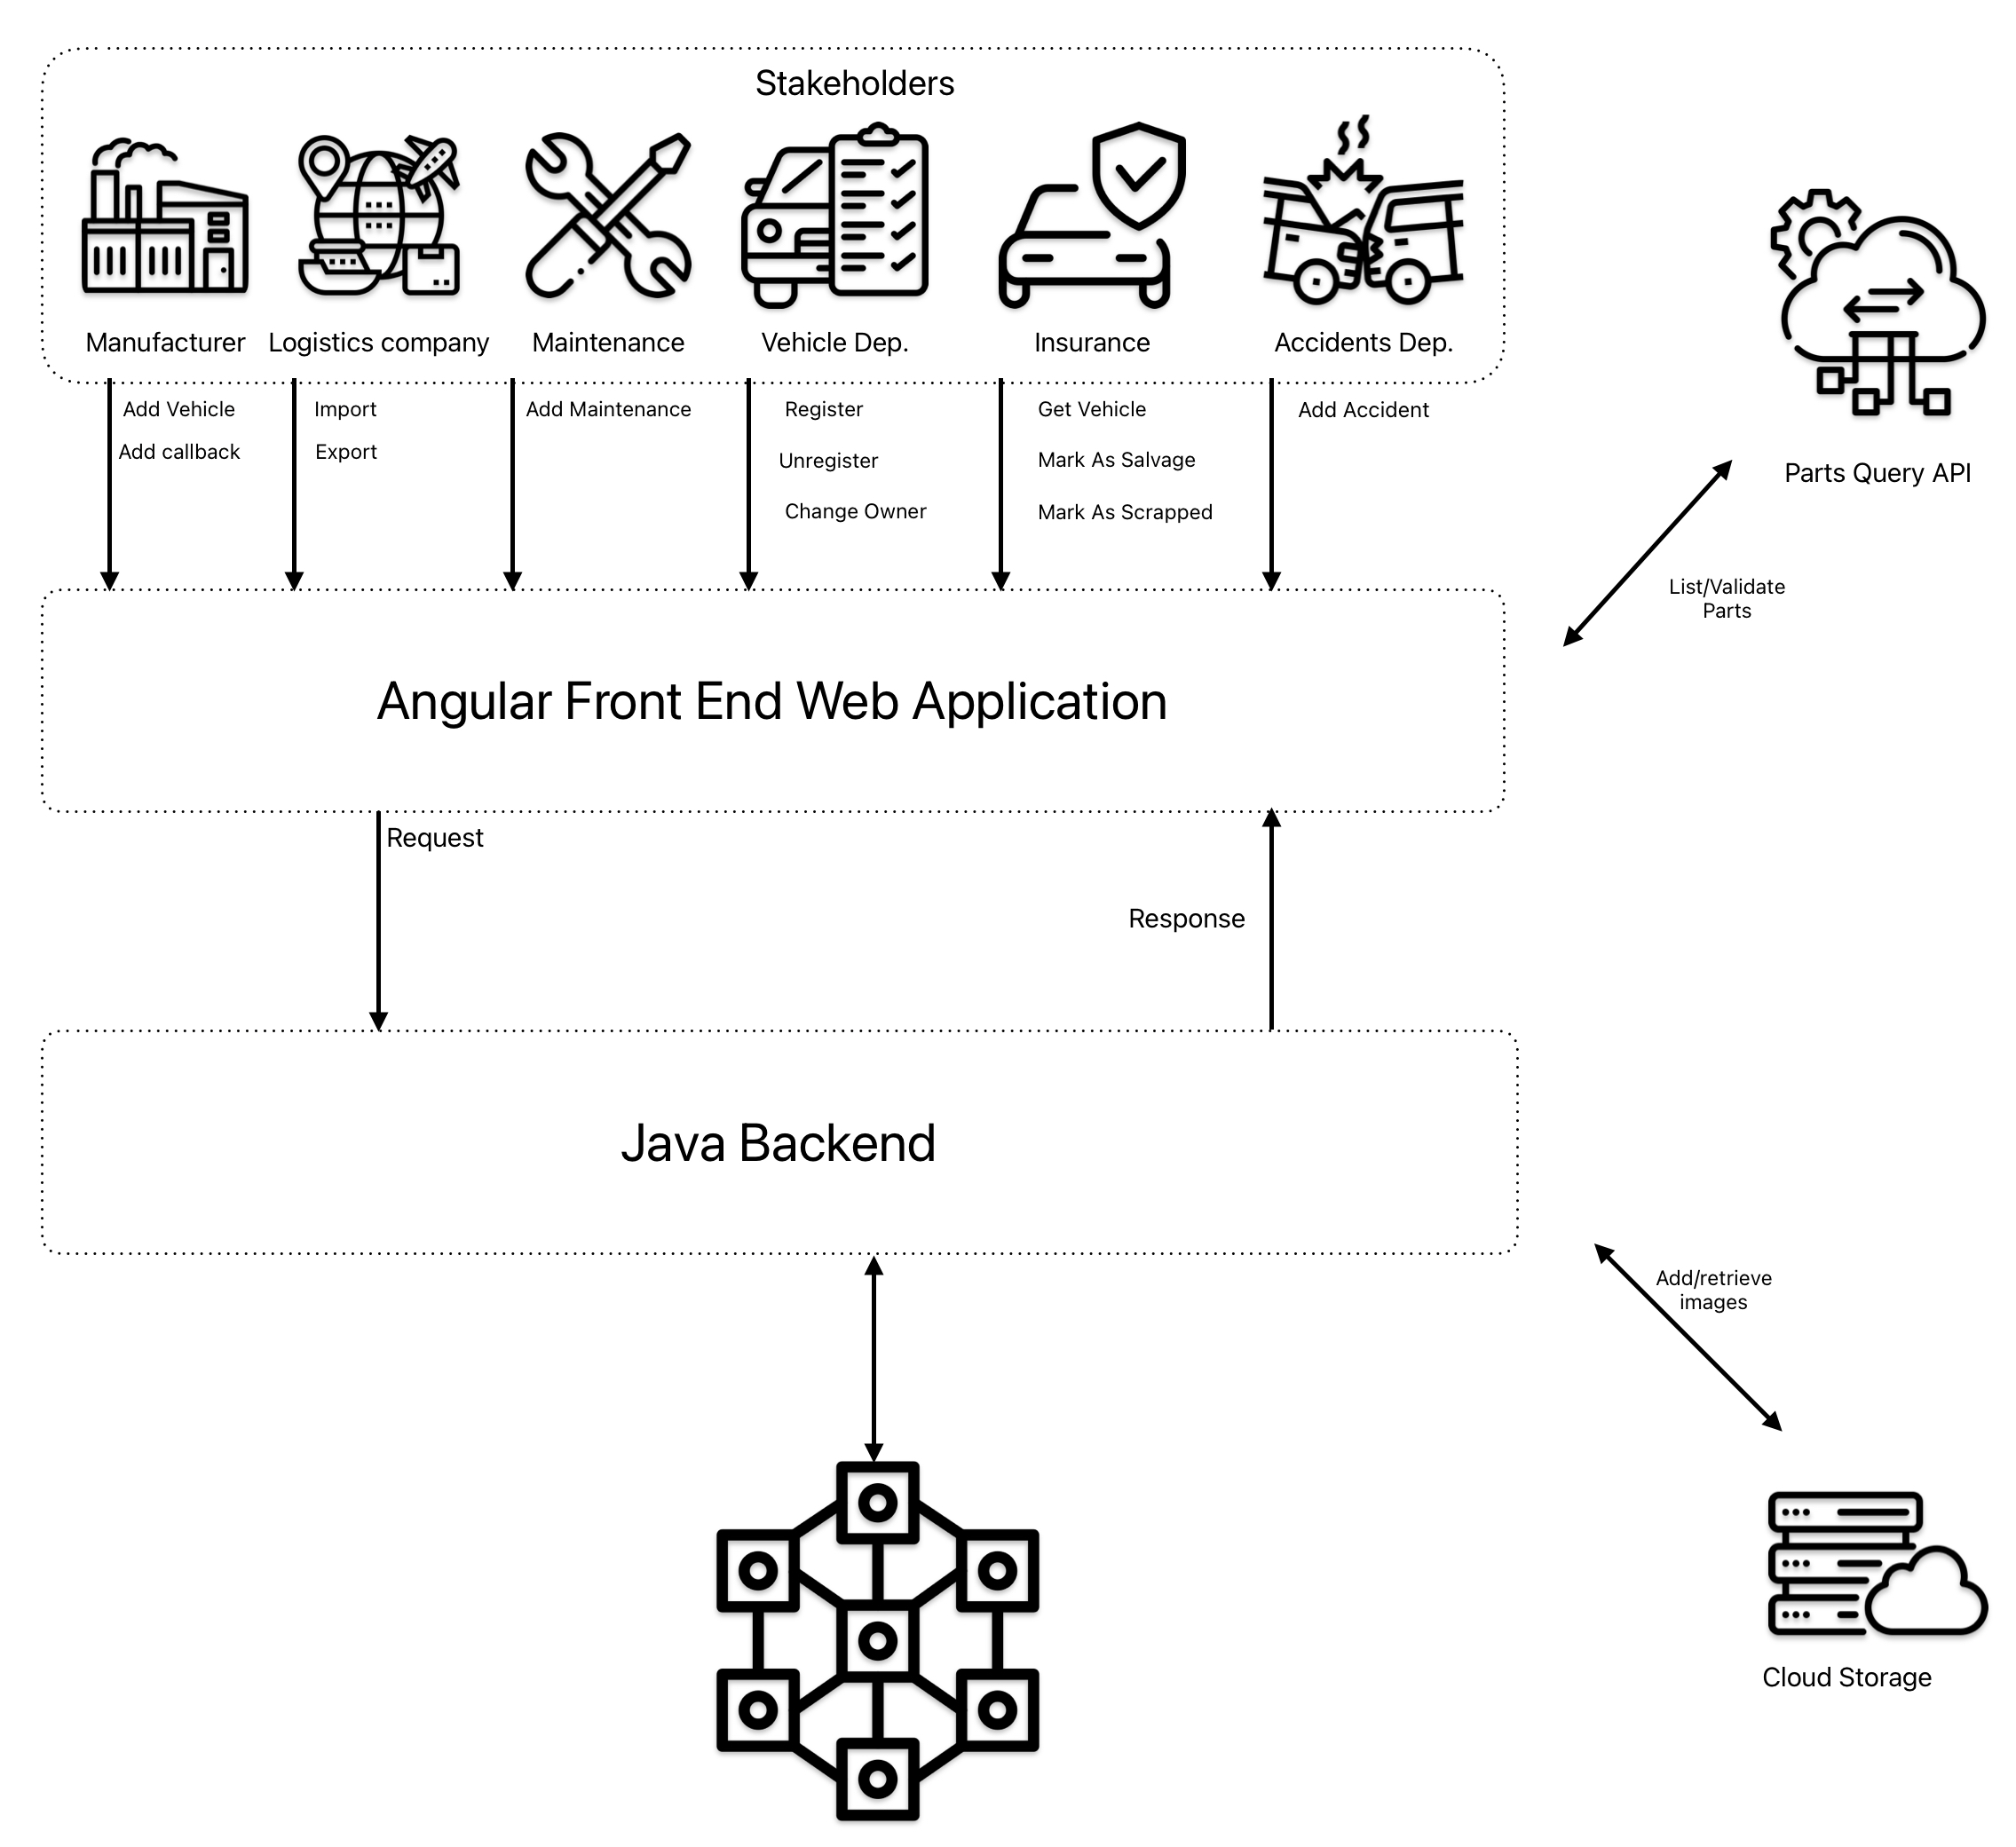
\includegraphics[width=\linewidth]{figures/sys-framework}
	\caption{System Framework.}
	\label{fig:sys-framework}
\end{figure}
The framework has six main stakeholders with specific operations for each. As figure \ref{fig:df-sys-framework} shows, the stakeholders are:
\begin{enumerate}
	\item Manufacturer, which can add new vehicles to the network and add vehicle callbacks.
	\item Logistics company, which has import and export operations.
	\item Maintenance shop, and it can only add new maintenance records.
	\item Vehicle department has three operations; register vehicles, unregister vehicles, change vehicle ownership.
	\item Insurance company, it can mark a vehicle as scrapped or salvaged and retrieve vehicle information.
	\item Accidents department has an operation to add vehicle accident records.
\end{enumerate}
\begin{figure}[H]
	\centering
	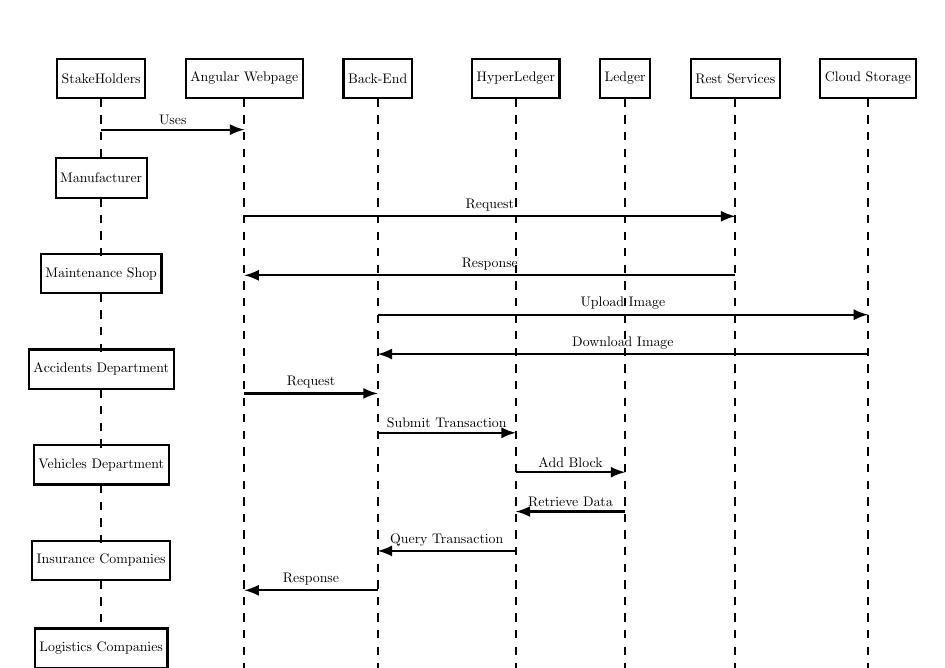
\begin{tikzpicture}[scale=0.5,transform shape]
		\tikzstyle{actor} = [draw, thick, minimum width=1cm, minimum height=1cm]
		\tikzstyle{message} = [draw, thick, -latex]
		\tikzstyle{instance} = [draw, thick, dashed, minimum height=6cm]

		\node[actor] (StakeHolder) {StakeHolders};
		\node[actor, below=1.5cm of StakeHolder] (Manufacturer) {Manufacturer};
		\node[actor, below=1.4 of Manufacturer] (Maintenance) {Maintenance Shop};
		\node[actor, below=1.4 of Maintenance] (Accidents) {Accidents Department};
		\node[actor, below=1.4 of Accidents] (Vehicles) {Vehicles Department};
		\node[actor, below=1.4 of Vehicles] (Insurance) {Insurance Companies};
		\node[actor, below=1.2 of Insurance] (Logistics) {Logistics Companies};
		\node[actor, right=1cm of StakeHolder] (Webpage) {Angular Webpage};
		\node[actor, right=1cm of Webpage] (BackEnd) {Back-End};
		\node[actor, right=1.5cm of BackEnd] (HyperLedger) {HyperLedger};
		\node[actor, right=1cm of HyperLedger] (Ledger) {Ledger};
		\node[actor, right=1cm of Ledger] (RestServices) {Rest Services};
		\node[actor, right=1cm of RestServices] (CloudStorage) {Cloud Storage};

		\draw[instance] (StakeHolder) -- ++(0,-2);
		\draw[instance] (Manufacturer) -- ++(0,-2);
		\draw[instance] (Maintenance) -- ++(0,-2);
		\draw[instance] (Accidents) -- ++(0,-2);
		\draw[instance] (Vehicles) -- ++(0,-2);
		\draw[instance] (Insurance) -- ++(0,-1.65);
		\draw[instance] (Webpage) -- ++(0,-15);
		\draw[instance] (BackEnd) -- ++(0,-15);
		\draw[instance] (HyperLedger) -- ++(0,-15);
		\draw[instance] (Ledger) -- ++(0,-15);
		\draw[instance] (RestServices) -- ++(0,-15);
		\draw[instance] (CloudStorage) -- ++(0,-15);

		\draw[message] ($(StakeHolder)-(0,1.3)$) -- ($(Webpage)-(0,1.3)$) node[midway, above] {Uses};
		\draw[message] ($(Webpage)-(0,8)$) -- ($(BackEnd)-(0,8)$) node[midway, above] {Request};
		\draw[message] ($(BackEnd)-(0,13)$) -- ($(Webpage)-(0,13)$) node[midway, above] {Response};
		\draw[message] ($(BackEnd)-(0,9)$) -- ($(HyperLedger)-(0,9)$) node[midway, above] {Submit Transaction};
		\draw[message] ($(HyperLedger)-(0,12)$) -- ($(BackEnd)-(0,12)$) node[midway, above] {Query Transaction};
		\draw[message] ($(Webpage)-(0,3.5)$) -- ($(RestServices)-(0,3.5)$) node[midway, above] {Request};
		\draw[message] ($(RestServices)-(0,5)$) -- ($(Webpage)-(0,5)$) node[midway, above] {Response};
		\draw[message] ($(HyperLedger)-(0,10)$) -- ($(Ledger)-(0,10)$) node[midway, above] {Add Block};
		\draw[message] ($(Ledger)-(0,11)$) -- ($(HyperLedger)-(0,11)$) node[midway, above] {Retrieve Data};
		\draw[message] ($(BackEnd)-(0,6)$) -- ($(CloudStorage)-(0,6)$) node[midway, above] {Upload Image};
		\draw[message] ($(CloudStorage)-(0,7)$) -- ($(BackEnd)-(0,7)$) node[midway, above] {Download Image};

	\end{tikzpicture}
	\caption{Framework Dataflow.}
	\label{fig:df-sys-framework}
\end{figure}

\begin{table}[H]
	\caption{Chaincode validations.}
	\label{tab:chaincode-validations}
	\tiny
	\begin{tabularx}{\linewidth}{X|X|X}
		\toprule
		Stakeholder        & Chaincode        & Validations
		\\
		\toprule
		Manufacturer         & Create Vehicle   &  VIN is unique. \newline
		All initial data exist (Color, Country of origin, Production year, Model). \\
		\cmidrule{2-3}
		& Create Callback  & -                                                                                                       \\
		\midrule
		Logistic             & Import           & Vehicle is exported. \newline Vehicle exists in the same country. \newline Valid 
		Odometer.
		\\
		\cmidrule{2-3}
		& Export           & Vehicle not registered to an owner. \newline Valid Odometer.                                            \\
		\midrule
		Accidents Department & -                & -
		\\
		\midrule
		Vehicles Department  & Register         & Not registered to an owner. \newline Vehicle is imported. \newline Valid Odometer.
		\\
		\cmidrule{2-3}
		& Unregister       & Registered to an owner. \newline Valid Odometer.                                                        \\
		\cmidrule{2-3}
		& Change Ownership & Registered to an owner. \newline Seller is the owner. \newline Valid Odometer.                          \\
		\midrule
		Maintenance          & Add Maintenance  & Valid Odometer. \newline Genuine Part: \newline Have serial number. \newline
		Authenticity verified.     \\
		\midrule
		Insurance companies  & -                & -
		\\
		\bottomrule
	\end{tabularx}
\end{table}
As table \ref{tab:chaincode-validations}
shows, the framework has a set of validations for each type of stakeholders to ensure the validity of the transactions before
adding them to the ledger. These validations are the cornerstone of the framework, so every endorsing peer will have its chaincode deployed
on separate container or server to ensure it is security and integrity. Finally, endorsement is based on the majority consensus method and
the transaction is considered valid only if the initiation peer received approvals from at least 50\% of the network.
\begin{figure}[H]
	\centering
	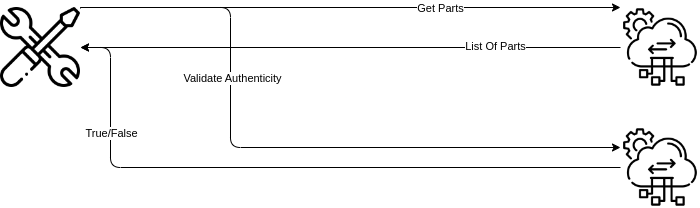
\includegraphics[width=\linewidth]{figures/parts-service-wf}
	\caption{Parts Query Service WorkFlow.}
	\label{fig:parts-query-wf}
\end{figure}

As figure \ref{fig:parts-query-wf}
shows, the framework uses a restful API to communicate with Parts Query API which is a Restful service deployed by vehicle
manufacturers with two endpoints to enable the framework to retrieve vehicles list of replacement parts and validate parts serial number in
case the manufacturer stated that it has a serial number. 


The framework is built on HL fabric framework as a hybrid BC where only users who the sufficient permissions can
add transactions based on their given role. To ensure transparency, vehicles reports are publicly available, and any individual
can query the data of any vehicle using its VIN without the need for credentials. 

\begin{figure}[H]
\centering
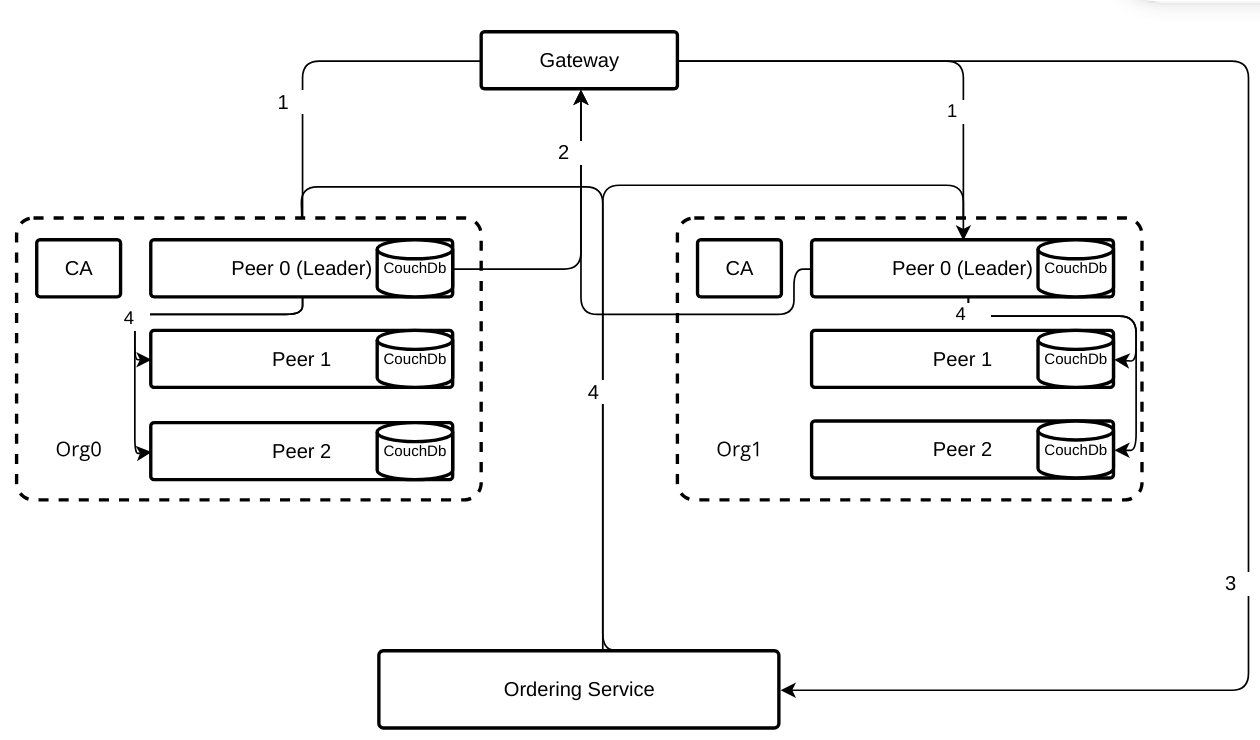
\includegraphics[width=\linewidth]{figures/hyper-ledger-flow}
\caption{Hyper Ledger Transaction Flow.}
\label{fig:hyper-ledger-wf}
\end{figure}
As figure~\ref{fig:hyper-ledger-wf}
show, the transaction moves in multiple stages before it is committed and we will dive into the flow as:
\begin{enumerate}
\item When the gateway receives the transaction request, it sends transaction proposal to the endorsing peers.
\item the endorsing peers simulate and validate the transaction, then it sends proposal response to the gateway.
\item when the gateway receives enough number of approvals it sends the transaction to the ordering service.
\item the ordering service maintains the transactions in a chronological order and when new block conditions are satisfied it sends
the new block to all peers to be committed.
\item the new block is now committed into the ledger.
\end{enumerate}
To enhance the performance of the peers and decrease the size of the transactions, an external
CouchDb is used to store the vehicle images. The images are encrypted using a unique cryptographic key generated for each
image, then its encrypted using base64 before uploading it to the external DB. The ledger will only contain the
image id the CouchDb and the decryption key, these measures ensures that images cannot be altered or modified if
a malicious party got access to the external DB. Moreover, the framework uses several security methods namely: spring security
with Json Web Token to control user's authentication and authorization, nginx server to manage the load balancing between server
nodes and prevent attacks such as Denial of Service (DoS), and the use of Transport Layer Security
(TLS) to secure all communications within the framework. Finally, the implementation of these methods ensures the framework security and
integrity. 

\section{Results and Discussion}
Experiment evaluation is a crucial step to determine the performance and applicability of our framework in the automotive industry. Through
systematic testing and evaluation our goal is to identify performance bottlenecks and areas of potential improvements to demonstrate the
solution feasibility for a real-world enterprise level applications In this section we will delve into the details of our experiments and
results using two benchmarking tools: HL Caliper and HL Tape. The use of these tools allows for a better understanding of performance under
different conditions and configurations.

\subsection{Experimental Setup}

\subsubsection{Testing Environment}
All experiments were performed on google cloud compute engine instance with the following specifications:
\begin{enumerate}
	\item 16 core CPU (32 virtual cores)
	\item 72 GB RAM
	\item Ubuntu 24.04
	\item X86/64 architecture
\end{enumerate}

\subsubsection{HL Fabric configuration}
Fabric provides several configurations that can be modified to achieve an optimal performance for different use cases, for our
framework
we set them as following:
\begin{enumerate}
	\item  TLS enabled to secure the network communications
	\item State database is CouchDb
	\item Consensus using Raft
	\item BatchTimeout (Block time) 2 seconds
	\item MaxMessageCount is 500
	\item Number of orderers is 3
\end{enumerate}

\subsubsection{Framework deployment}
All framework parts were deployed to docker compose in one network, each organization consists of at least one peer and each peer depends
on a chaincode and database container.
In case of multiple peers in an organization, there is two types of deployments for peers: leader
and followers were only the leader has a chaincode node and handle all external communication.
In the second type, all peers have chaincode nodes and load is balanced among them.
We chose the second type for our evaluation to measure the additional peer impact on the performance.
Finally, there must be at least one orderer node however, it is recommended to have at least 5 ordering nodes in the network to
have fault tolerance with 40\% of nodes are down and achieve a valid consensus and leader election, for our evaluation three orderer
nodes where deployed.

\subsection{Experiment Result}\label{subsec:experiment-result}
The framework was evaluated on the CreateVehicle and QueryVehicle chaincodes, based on the framework validation we can repeat the
CreateVehicle invocation any number of times as long as the VIN is not duplicated, Universally Unique Identifier (UUID) was
used to generate a unique one each time.
For QueryVehicle, a Vehicle with VIN “testVehicle” was added to the chain at the network setup to be queried.
Furthermore, the framework was benchmarked with 2 different variables: Number of transactions per second and the number of
organizations
and peers.
Finally, the benchmarking tools were Caliper and Tape which were introduced by HL foundation as benchmarking tools
to support Fabric and other projects.

\subsubsection{Performance Evaluation Using HL Caliper}\label{subsubsec:hlceval}
Caliper was intended to evaluate BC systems such as Fabric in production or pre–production stages such as: System Integration Testing (SIT)
and User Acceptance Testing (UAT) to provide an estimate of the system performance in production after go-live stage. The benchmark results
consist of several metrics with the ability to monitor system resources such as RAM, CPU, network traffic, and disk read/write, and the
metrics are:
\begin{enumerate}
	\item Send Rate TPS: the actual TPS caliper achieved.
	\item Latency: the amount of time it took a new transaction to be added to the chain.
	\item Throughput TPS: the number of transactions the framework can process and add to the chain per second.
\end{enumerate}
For Caliper configuration the values were:
\begin{enumerate}
	\item txDuration (benchmark duration): 30 seconds and 90 seconds for CreateVehicle and QueryVehicle, respectively.
	\item rateControl (transaction send method): fixed-rate
\end{enumerate}
\begin{table}[H]
	\centering
	\footnotesize
	\tiny
	\caption{Performance Metrics for CreateVehicle chaincode}
	\label{tab:createvehiclepm}
	\begin{tabularx}{\textwidth}
	{>{\centering\arraybackslash}X|>{\centering\arraybackslash}X|>{\centering\arraybackslash}X|>{\centering\arraybackslash}X|
			>{\centering\arraybackslash}X|>{\centering\arraybackslash}X|>{\centering\arraybackslash}X|>{\centering\arraybackslash}X|
			>{\centering\arraybackslash}X|>{\centering\arraybackslash}X}
		\toprule
		\textbf{No. Orgs} & \textbf{No. Peers} & \textbf{TPS} & \textbf{Succ} & \textbf{Success Rate} &
		\textbf{Send Rate TPS} & \textbf{Max Latency (s)} & \textbf{Min Latency (s)} & \textbf{Avg Latency (s)} &
		\textbf{Throughput TPS} \\
		\midrule
		\multirow{8}{*}{\textbf{5}} & \multirow{4}{*}{\textbf{1}} & 80 & 2401.00 & 100.00\%
		& 80.00  & 7.50  & 0.82 & 3.35  & 73.00  \\
		\cline{3-10}
		& & 90 & 2701.00 & 100.00\%
		& 90.10 & 16.25 & 1.15 & 6.79 & 71.40
		\\
		\cline{3-10}
		& & 100 & 3001.00 & 100.00\%
		& 100.10 & 23.88 & 1.38 & 11.26 & 71.80
		\\
		\cline{3-10}
		& & 120 & 3601.00 & 100.00\%
		& 120.10 & 35.49 & 1.60 & 20.82 & 69.70
		\\
		\cline{2-10}
		& \multirow{4}{*}{\textbf{2}} & 80 & 2400.00 & 100.00\%
		& 80.00 & 3.56 & 0.88 & 2.09 & 77.50
		\\
		\cline{3-10}
		& & 90 & 2694.00 & 100.00\%
		& 89.70 & 5.37 & 1.06 & 2.94 & 82.90
		\\
		\cline{3-10}
		& & 100 & 2895.00 & 100.00\%
		& 96.50 & 6.12 & 1.01 & 3.39 & 91.90
		\\
		\cline{3-10}
		& & 120 & 2895.00 & 100.00\%
		& 96.30 & 6.59 & 1.11 & 3.58 & 92.20
		\\
		\midrule
		\multirow{4}{*}{\textbf{7}} & \multirow{4}{*}{\textbf{1}} & 80 & 2401.00 & 100.00\%
		& 80.00  & 20.80 & 1.35 & 6.62  & 61.70  \\
		\cline{3-10}
		& & 90 & 2700.00 & 100.00\%
		& 90.00 & 26.26 & 1.70 & 10.69 & 60.30
		\\
		\cline{3-10}
		& & 100 & 3001.00 & 100.00\%
		& 100.10 & 33.30 & 1.93 & 15.88 & 59.30
		\\
		\cline{3-10}
		& & 120 & 3601.00 & 100.00\%
		& 120.10 & 43.21 & 2.02 & 25.17 & 57.90
		\\
		\midrule
		\multirow{4}{*}{\textbf{10}} & \multirow{4}{*}{\textbf{1}} & 80 & 2401.00 & 100.00\%
		& 80.00  & 33.68 & 2.65 & 19.63 & 43.00  \\
		\cline{3-10}
		& & 90 & 2701.00 & 100.00\%
		& 90.00 & 39.38 & 2.82 & 25.53 & 43.20
		\\
		\cline{3-10}
		& & 100 & 3001.00 & 100.00\%
		& 100.00 & 48.97 & 3.29 & 31.70 & 42.60
		\\
		\cline{3-10}
		& & 120 & 3601.00 & 100.00\%
		& 120.10 & 66.15 & 3.32 & 44.06 & 41.70
		\\
		\bottomrule
	\end{tabularx}
\end{table}
\begin{figure}[H]
	\begin{center}
		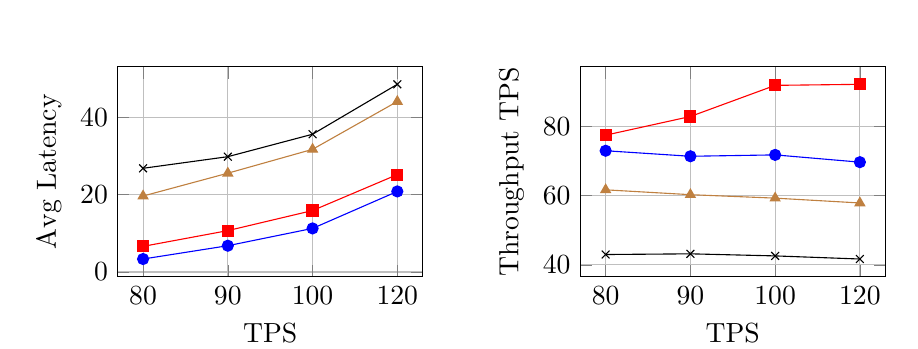
\begin{tikzpicture}
			\begin{groupplot}[
				group style={
					group name=my plots,
					group size=2 by 1,
					xlabels at=edge bottom,
					ylabels at=edge left,
					horizontal sep=2cm,
					vertical sep=3cm,
				},
				symbolic x coords={80, 90, 100, 120},
				xtick=data,
				width=0.45\linewidth,
				height=0.35\linewidth,
				grid=major
			]
				% Avg Latency Plot
				\nextgroupplot[legend to name=testLegend, xlabel={TPS}, ylabel={Avg Latency}]
				\addplot[blue, mark=*] coordinates {(80, 3.35) (90, 6.79) (100, 11.26) (120, 20.82)};
				\addplot[red, mark=square*] coordinates {(80, 6.62) (90, 10.69) (100, 15.88) (120, 25.17)};
				\addplot[brown, mark=triangle*] coordinates {(80, 19.63) (90, 25.53) (100, 31.70) (120, 44.06)};
				\addplot[black, mark=x] coordinates {(80, 26.80) (90, 29.80) (100, 35.60) (120, 48.50)};

				% Throughput Plot
				\nextgroupplot[legend to name=testLegend, xlabel={TPS}, ylabel={Throughput TPS}]
				\addplot[blue, mark=*] coordinates {(80, 73.00) (90, 71.40) (100, 71.80) (120, 69.70)};
				\addplot[red, mark=square*] coordinates {(80, 77.50) (90, 82.90) (100, 91.90) (120, 92.20)};
				\addplot[brown, mark=triangle*] coordinates {(80, 61.70) (90, 60.30) (100, 59.30) (120, 57.90)};
				\addplot[black, mark=x] coordinates {(80, 43.00) (90, 43.20) (100, 42.60) (120, 41.70)};

				% Legend Entries
				\addlegendentry{5 Orgs 1 Peer}
				\addlegendentry{5 Orgs 2 Peers}
				\addlegendentry{7 Orgs 1 Peer}
				\addlegendentry{10 Orgs 1 Peer}
			\end{groupplot}
		\end{tikzpicture}
		\ref{testLegend}
		\caption{Performance Metrics for CreateVehicle chaincode.}
		\label{fig:createvehiclepm}
	\end{center}
\end{figure}
As figure \ref{fig:createvehiclepm}
and table \ref{tab:createvehiclepm}
shows that average latency increases with TPS, with 10 Orgs 1 Peer having the highest latency, reaching 48.5
seconds at 120 TPS, while 5 Orgs 1 Peer maintains the lowest latency, rising from 3.35 seconds at 80 TPS to 20.82 seconds at 120 TPS.
Throughput trends reveal that 5 Orgs 2 Peers sustains the highest rates, achieving up to 92.2 TPS at 120 TPS with a
32.2\% increase compared to 5 Orgs 1 Peer, suggesting that additional peers per organization can support higher transaction volumes. In
contrast, 10 Orgs 1 Peer consistently exhibits the lowest throughput, dropping to 41.7 TPS at 120 TPS, indicating that organizational
and peer configuration significantly impact latency and throughput capabilities if computational power and hardware specification is not
sufficient.
\begin{table}[H]
	\centering
	\footnotesize
	\tiny
	\caption{Performance Metrics for QueryVehicle chaincode.}
	\label{tab:queryvehiclepm}
	\begin{tabularx}{\textwidth}
	{>{\centering\arraybackslash}X|>{\centering\arraybackslash}X|>{\centering\arraybackslash}X|>{\centering\arraybackslash}X|
			>{\centering\arraybackslash}X|>{\centering\arraybackslash}X|>{\centering\arraybackslash}X|>{\centering\arraybackslash}X|
			>{\centering\arraybackslash}X|>{\centering\arraybackslash}X}
		\toprule
		\textbf{No. Orgs} & \textbf{No. Peers} & \textbf{TPS} & \textbf{Succ} & \textbf{Success Rate} &
		\textbf{Send Rate TPS} & \textbf{Max Latency (s)} & \textbf{Min Latency (s)} & \textbf{Avg Latency (s)} &
		\textbf{Throughput TPS} \\
		\midrule
		\multirow{4}{*}{\textbf{5}} & \multirow{2}{*}{\textbf{1}} & 130 & 7613 & 100.00\%
		& 126.9  & 6.33  & 1.00  & 3.48  & 120.2  \\
		\cline{3-10}
		& & 140 & 7657 & 100.00\%
		& 127.5 & 6.06 & 1.15 & 3.64 & 121.3
		\\
		\cline{2-10}
		& \multirow{2}{*}{\textbf{2}} & 130 & 6977 & 100.00\%
		& 116.3 & 3.79 & 0.93 & 2.74 & 114.4
		\\
		\cline{3-10}
		& & 140 & 7113 & 100.00\%
		& 118.5 & 3.78 & 0.96 & 2.70 & 116.4
		\\
		\midrule
		\multirow{2}{*}{\textbf{7}} & \multirow{2}{*}{\textbf{1}} & 130 & 6942 & 100.00\%
		& 115.7  & 11.25 & 1.66  & 5.36  & 107.2  \\
		\cline{3-10}
		& & 140 & 6635 & 100.00\%
		& 110.6 & 8.97 & 1.84 & 4.66 & 104.4
		\\
		\midrule
		\multirow{2}{*}{\textbf{10}} & \multirow{2}{*}{\textbf{1}} & 130 & 6496 & 100.00\%
		& 108.3  & 48.42 & 3.19  & 31.42 & 64.1  \\
		\cline{3-10}
		& & 140 & 6486 & 100.00\%
		& 108.1 & 43.15 & 3.19 & 29.00 & 67.2
		\\
		\bottomrule
	\end{tabularx}
\end{table}
\begin{figure}[H]
	\begin{center}
		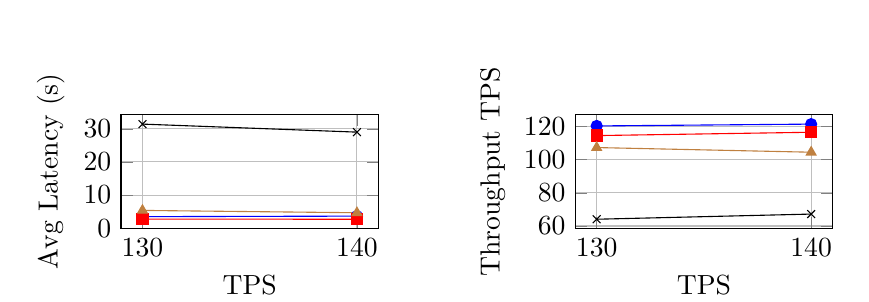
\begin{tikzpicture}
			\begin{groupplot}[
				group style={
					group name=my plots,
					group size=2 by 1,
					xlabels at=edge bottom,
					ylabels at=edge left,
					horizontal sep=2.5cm,
					vertical sep=1cm,
				},
				symbolic x coords={130, 140},
				xtick=data,
				width=0.4\linewidth,
				height=0.25\linewidth,
				grid=major
			]
				% Avg Latency Plot
				\nextgroupplot[legend to name=testLegend1, xlabel={TPS}, ylabel={Avg Latency (s)}]
				\addplot[blue, mark=*] coordinates {(130, 3.48) (140, 3.64)};
				\addplot[red, mark=square*] coordinates {(130, 2.74) (140, 2.70)};
				\addplot[brown, mark=triangle*] coordinates {(130, 5.36) (140, 4.66)};
				\addplot[black, mark=x] coordinates {(130, 31.42) (140, 29.00)};

				% Throughput Plot
				\nextgroupplot[legend to name=testLegend1, xlabel={TPS}, ylabel={Throughput TPS}]
				\addplot[blue, mark=*] coordinates {(130, 120.2) (140, 121.3)};
				\addplot[red, mark=square*] coordinates {(130, 114.4) (140, 116.4)};
				\addplot[brown, mark=triangle*] coordinates {(130, 107.2) (140, 104.4)};
				\addplot[black, mark=x] coordinates {(130, 64.1) (140, 67.2)};

				% Legend Entries
				\addlegendentry{5 Orgs 1 Peer}
				\addlegendentry{5 Orgs 2 Peers}
				\addlegendentry{7 Orgs 1 Peer}
				\addlegendentry{10 Orgs 1 Peer}
			\end{groupplot}
		\end{tikzpicture}
		\ref{testLegend1}
		\caption{Performance Metrics for QueryVehicle chaincode.}
		\label{fig:queryvehiclepm}
	\end{center}
\end{figure}
As figure \ref{fig:queryvehiclepm} and table \ref{tab:queryvehiclepm}
show, the average latency varies notably, with 5 Orgs 1 Peer and 5 Orgs 2 Peers
configurations achieving
relatively
low latency (around 3-4 seconds), while 10 Orgs 1 Peer shows a significantly higher latency, exceeding 29 seconds. Throughput values are
also impacted by number of organizations and peers, with 5 Orgs 1 Peer and 5 Orgs 2 Peers configurations achieving the highest throughput
(around 120 TPS), and 10 Orgs 1 Peer experiencing lower throughput (64-67 TPS). These observations suggest that adding peers within
organizations may reduce latency and improve throughput, while having more organizations without additional resources can impact performance
negatively.

\subsubsection{Chaincode Evaluation}
\begin{table}[H]
	\centering
	\footnotesize
	\tiny
	\caption{Resource Usage for Chaincode nodes on CreateVehicle chaincode.}
	\label{tab:createvehiclechaincoderu}
	\begin{tabularx}{\textwidth}
	{>{\centering\arraybackslash}X|>{\centering\arraybackslash}X|>{\centering\arraybackslash}X|>{\centering\arraybackslash}X|
			>{\centering\arraybackslash}X|>{\centering\arraybackslash}X|>{\centering\arraybackslash}X}
		\toprule
		\textbf{No. Orgs} & \textbf{No. Peers} & \textbf{TPS} & \textbf{CPU\% (avg)} & \textbf{Memory (avg) [MB]} &
		\textbf{Traffic In (avg) [MB]} & \textbf{Traffic Out (avg) [MB]} \\
		\midrule
		\multirow{8}{*}{\textbf{5}} & \multirow{4}{*}{\textbf{1}}
		& 80 & 0.075 & 567.600 & 4.280 & 2.386 \\
		\cline{3-7}
		& & 90 & 0.066 & 576.800 & 4.762 &
		2.628 \\
		\cline{3-7}
		& & 100 & 0.072 & 577.200 & 5.256 &
		2.886 \\
		\cline{3-7}
		& & 120 & 0.072 & 577.200 & 5.256 &
		2.886 \\
		\cline{2-7}
		& \multirow{4}{*}{\textbf{2}}
		& 80 & 0.043 & 572.100 & 2.160 & 1.214
		\\
		\cline{3-7}
		& & 90 & 0.048 & 576.100 & 2.388 &
		1.328 \\
		\cline{3-7}
		& & 100 & 0.054 & 584.500 & 2.560 &
		1.415 \\
		\cline{3-7}
		& & 120 & 0.054 & 584.500 & 2.560 &
		1.415 \\
		\midrule
		\multirow{4}{*}{\textbf{7}} & \multirow{4}{*}{\textbf{1}}
		& 80 & 0.056 & 586.571 & 4.006 & 2.227 \\
		\cline{3-7}
		& & 90 & 0.053 & 588.857 & 4.470 &
		2.453 \\
		\cline{3-7}
		& & 100 & 0.060 & 589.000 & 4.967 &
		2.711 \\
		\cline{3-7}
		& & 120 & 0.060 & 589.000 & 4.967 &
		2.711 \\
		\midrule
		\multirow{4}{*}{\textbf{10}} & \multirow{4}{*}{\textbf{1}}
		& 80 & 0.05 & 563.30 & 4.12                           & 2.24
		\\
		\cline{3-7}
		& & 90 & 0.048 & 568.200 & 4.644 &
		2.523 \\
		\cline{3-7}
		& & 100 & 0.049 & 568.500 & 5.168 &
		2.811 \\
		\cline{3-7}
		& & 120 & 0.049 & 568.500 & 5.168 &
		2.811 \\
		\bottomrule
	\end{tabularx}
\end{table}
\begin{figure}[H]
	\begin{center}
		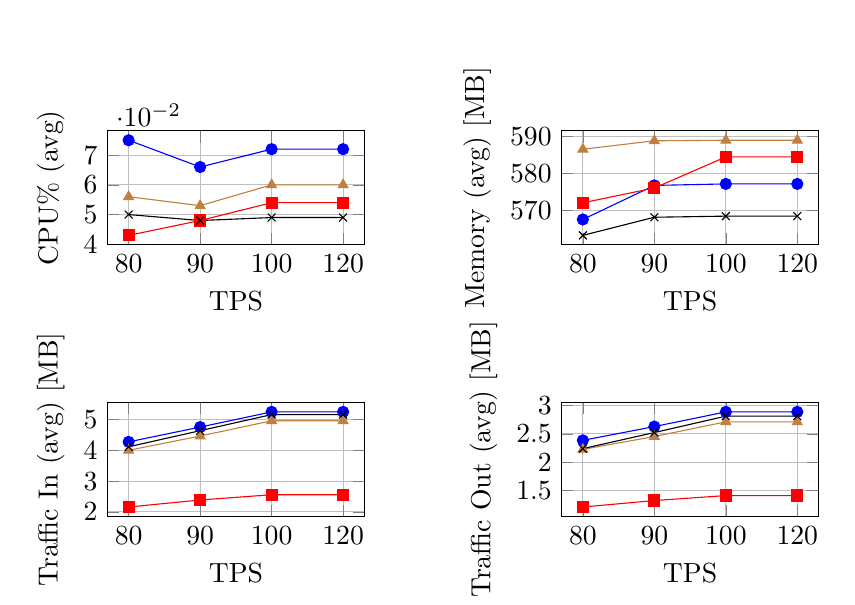
\begin{tikzpicture}
			\begin{groupplot}[
				group style={
					group name=my plots,
					group size=2 by 2,
					xlabels at=edge bottom,
					ylabels at=edge left,
					horizontal sep=2.5cm,
					vertical sep=2cm,
				},
				symbolic x coords={80, 90, 100, 120},
				xtick=data,
				width=0.4\linewidth,
				height=0.25\linewidth,
				grid=major
			]

				% CPU Usage Plot
				\nextgroupplot[legend to name=testLegend2, xlabel={TPS}, ylabel={CPU\% (avg)}]
				\addplot[blue, mark=*] coordinates {(80, 0.075) (90, 0.066) (100, 0.072) (120, 0.072)};
				\addplot[red, mark=square*] coordinates {(80, 0.043) (90, 0.048) (100, 0.054) (120, 0.054)};
				\addplot[brown, mark=triangle*] coordinates {(80, 0.056) (90, 0.053) (100, 0.060) (120, 0.060)};
				\addplot[black, mark=x] coordinates {(80, 0.05) (90, 0.048) (100, 0.049) (120, 0.049)};

				% Memory Usage Plot
				\nextgroupplot[legend to name=testLegend2, xlabel={TPS}, ylabel={Memory (avg) [MB]}]
				\addplot[blue, mark=*] coordinates {(80, 567.600) (90, 576.800) (100, 577.200) (120, 577.200)};
				\addplot[red, mark=square*] coordinates {(80, 572.100) (90, 576.100) (100, 584.500) (120, 584.500)};
				\addplot[brown, mark=triangle*] coordinates {(80, 586.571) (90, 588.857) (100, 589.000) (120, 589.000)};
				\addplot[black, mark=x] coordinates {(80, 563.300) (90, 568.200) (100, 568.500) (120, 568.500)};

				% Traffic In Plot
				\nextgroupplot[legend to name=testLegend2, xlabel={TPS}, ylabel={Traffic In (avg) [MB]}]
				\addplot[blue, mark=*] coordinates {(80, 4.280) (90, 4.762) (100, 5.256) (120, 5.256)};
				\addplot[red, mark=square*] coordinates {(80, 2.160) (90, 2.388) (100, 2.560) (120, 2.560)};
				\addplot[brown, mark=triangle*] coordinates {(80, 4.006) (90, 4.470) (100, 4.967) (120, 4.967)};
				\addplot[black, mark=x] coordinates {(80, 4.120) (90, 4.644) (100, 5.168) (120, 5.168)};

				% Traffic Out Plot
				\nextgroupplot[legend to name=testLegend2, xlabel={TPS}, ylabel={Traffic Out (avg) [MB]}]
				\addplot[blue, mark=*] coordinates {(80, 2.386) (90, 2.628) (100, 2.886) (120, 2.886)};
				\addplot[red, mark=square*] coordinates {(80, 1.214) (90, 1.328) (100, 1.415) (120, 1.415)};
				\addplot[brown, mark=triangle*] coordinates {(80, 2.227) (90, 2.453) (100, 2.711) (120, 2.711)};
				\addplot[black, mark=x] coordinates {(80, 2.240) (90, 2.523) (100, 2.811) (120, 2.811)};

				% Legend Entries
				\addlegendentry{5 Orgs 1 Peer}
				\addlegendentry{5 Orgs 2 Peers}
				\addlegendentry{7 Orgs 1 Peer}
				\addlegendentry{10 Orgs 1 Peer}
			\end{groupplot}
		\end{tikzpicture}
		\ref{testLegend2}
		\caption{Resource Usage for Chaincode nodes on CreateVehicle chaincode.}
		\label{fig:createvehiclechaincoderu}
	\end{center}
\end{figure}
As figure \ref{fig:createvehiclechaincoderu} and table \ref{tab:createvehiclechaincoderu}
shows, the chaincode nodes resource utilization for CreateVehicle chaincode.
CPU usage remains low, generally
under 0.08\%
, across all setups, with 5 Orgs 1 Peer showing the highest and 10 Orgs 1 Peer the lowest CPU demands. Memory usage stabilizes at around
570–590 MB, showing minimal increase as TPS grows, indicating that memory demands are relatively independent of TPS within this range.
Network traffic in and out, however, increases slightly with higher TPS, with inbound traffic ranging from 4 to 5.3 MB and outbound traffic
between 1.2 and 2.9 MB, with the 5 Orgs 1 Peer configuration consistently having the highest traffic as the load is the same across all
configurations. This analysis indicates that CPU and memory resources remain stable under varying TPS, while network traffic shows moderate
sensitivity to transaction load.
\begin{table}[H]
	\centering
	\footnotesize
	\tiny
	\caption{Resource Usage for Chaincode nodes on QueryVehicle chaincode.}
	\label{tab:queryvehiclechaincoderu}
	\begin{tabularx}{\textwidth}
	{>{\centering\arraybackslash}X|>{\centering\arraybackslash}X|>{\centering\arraybackslash}X|>{\centering\arraybackslash}X|
			>{\centering\arraybackslash}X|>{\centering\arraybackslash}X|>{\centering\arraybackslash}X}
		\toprule
		\textbf{No. Orgs} & \textbf{No. Peers} & \textbf{TPS} & \textbf{CPU\% (avg)} & \textbf{Memory (avg) [MB]} &
		\textbf{Traffic In (avg) [MB]} & \textbf{Traffic Out (avg) [MB]} \\
		\midrule
		\multirow{4}{*}{\textbf{5}} & \multirow{2}{*}{\textbf{1}}
		& 130 & 0.061 & 506.667 & 17.650 & 15.915 \\
		\cline{3-7}
		& & 140 & 0.053 & 577.600 & 10.940 &
		4.958 \\
		\cline{2-7}
		& \multirow{2}{*}{\textbf{2}}
		& 130 & 0.032 & 573.100 & 5.158 & 2.368
		\\
		\cline{3-7}
		& & 140 & 0.029 & 587.800 & 5.263 &
		2.416 \\
		\midrule
		\multirow{2}{*}{\textbf{7}} & \multirow{2}{*}{\textbf{1}}
		& 130 & 0.051 & 586.571 & 9.451 & 4.244 \\
		\cline{3-7}
		& & 140 & 0.040 & 589.143 & 9.107 &
		4.090 \\
		\midrule
		\multirow{2}{*}{\textbf{10}} & \multirow{2}{*}{\textbf{1}}
		& 130 & 0.033 & 563.600 & 9.207 & 4.089 \\
		\cline{3-7}
		& & 140 & 0.035 & 578.700 & 9.147 &
		4.055 \\
		\bottomrule
	\end{tabularx}
\end{table}
\begin{figure}[H]
	\begin{center}
		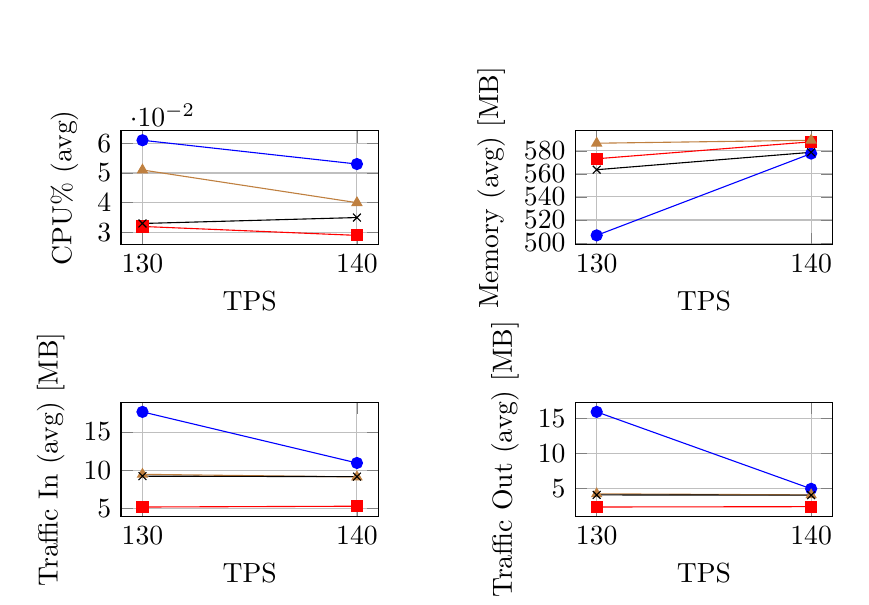
\begin{tikzpicture}
			\begin{groupplot}[
				group style={
					group name=my plots,
					group size=2 by 2,
					xlabels at=edge bottom,
					ylabels at=edge left,
					horizontal sep=2.5cm,
					vertical sep=2cm,
				},
				symbolic x coords={130, 140},
				xtick=data,
				width=0.4\linewidth,
				height=0.25\linewidth,
				grid=major
			]

				% CPU Usage Plot
				\nextgroupplot[legend to name=testLegend3, xlabel={TPS}, ylabel={CPU\% (avg)}]
				\addplot[blue, mark=*] coordinates {(130, 0.061) (140, 0.053)};
				\addplot[red, mark=square*] coordinates {(130, 0.032) (140, 0.029)};
				\addplot[brown, mark=triangle*] coordinates {(130, 0.051) (140, 0.040)};
				\addplot[black, mark=x] coordinates {(130, 0.033) (140, 0.035)};

				% Memory Usage Plot
				\nextgroupplot[legend to name=testLegend3, xlabel={TPS}, ylabel={Memory (avg) [MB]}]
				\addplot[blue, mark=*] coordinates {(130, 506.667) (140, 577.600)};
				\addplot[red, mark=square*] coordinates {(130, 573.100) (140, 587.800)};
				\addplot[brown, mark=triangle*] coordinates {(130, 586.571) (140, 589.143)};
				\addplot[black, mark=x] coordinates {(130, 563.600) (140, 578.700)};

				% Traffic In Plot
				\nextgroupplot[legend to name=testLegend3, xlabel={TPS}, ylabel={Traffic In (avg) [MB]}]
				\addplot[blue, mark=*] coordinates {(130, 17.650) (140, 10.940)};
				\addplot[red, mark=square*] coordinates {(130, 5.158) (140, 5.263)};
				\addplot[brown, mark=triangle*] coordinates {(130, 9.451) (140, 9.107)};
				\addplot[black, mark=x] coordinates {(130, 9.207) (140, 9.147)};

				% Traffic Out Plot
				\nextgroupplot[legend to name=testLegend3, xlabel={TPS}, ylabel={Traffic Out (avg) [MB]}]
				\addplot[blue, mark=*] coordinates {(130, 15.915) (140, 4.958)};
				\addplot[red, mark=square*] coordinates {(130, 2.368) (140, 2.416)};
				\addplot[brown, mark=triangle*] coordinates {(130, 4.244) (140, 4.090)};
				\addplot[black, mark=x] coordinates {(130, 4.089) (140, 4.055)};

				% Legend Entries
				\addlegendentry{5 Orgs 1 Peer}
				\addlegendentry{5 Orgs 2 Peers}
				\addlegendentry{7 Orgs 1 Peer}
				\addlegendentry{10 Orgs 1 Peer}
			\end{groupplot}
		\end{tikzpicture}
		\ref{testLegend3}
		\caption{Resource Usage for Chaincode nodes on QueryVehicle chaincode.}
		\label{fig:queryvehiclechaincoderu}
	\end{center}
\end{figure}
Figure \ref{fig:queryvehiclechaincoderu}
shows the chaincode nodes resource utilization for QueryVehicle chaincode, CPU usage remains low across all configurations,
indicating that CPU demand does not scale significantly with increased TPS load. Memory usage, however, is substantially higher, with values
reaching over 580 MB in some configurations, especially in setups with more organizations, like 10 Orgs 1 Peer. This suggests that higher
TPS demands increase memory requirements significantly. For network traffic, there is a noticeable drop in both inbound and outbound traffic
as TPS increases from 130 to 140, especially in the 5 Orgs 1 Peer setup. This could be explained by the direct relationship between TPS and
network traffic. Overall, the findings highlight that memory becomes a critical resource as transaction rates increase, while CPU and
network traffic show more stability under high load.

\subsubsection{Peers Evaluation}
\begin{table}[H]
	\centering
	\footnotesize
	\tiny
	\caption{Resource Usage for peers on CreateVehicle.}
	\label{tab:createvehiclepeerru}
	\begin{tabularx}{\textwidth}
	{>{\centering\arraybackslash}X|>{\centering\arraybackslash}X|>{\centering\arraybackslash}X|>{\centering\arraybackslash}X|
			>{\centering\arraybackslash}X|>{\centering\arraybackslash}X|>{\centering\arraybackslash}X}
		\toprule
		\textbf{No. Orgs} & \textbf{No. Peers} & \textbf{TPS} & \textbf{CPU\% (avg)} & \textbf{Memory (avg) [MB]} &
		\textbf{Traffic In (avg) [MB]} & \textbf{Traffic Out (avg) [MB]} \\
		\midrule
		\multirow{8}{*}{\textbf{5}} & \multirow{4}{*}{\textbf{1}}
		& 80 & 0.044 & 200.600 & 27.660 & 16.920 \\
		\cline{3-7}
		& & 90 & 0.045 & 199.200 & 31.040 &
		18.920 \\
		\cline{3-7}
		& & 100 & 0.044 & 202.000 & 34.400 &
		20.960 \\
		\cline{3-7}
		& & 120 & 0.044 & 224.400 & 41.180 &
		25.080 \\
		\cline{2-7}
		& \multirow{4}{*}{\textbf{2}}
		& 80 & 0.036 & 227.700 & 37.130 & 24.630
		\\
		\cline{3-7}
		& & 90 & 0.038 & 264.400 & 41.540 &
		27.490 \\
		\cline{3-7}
		& & 100 & 0.040 & 206.100 & 44.570 &
		29.470 \\
		\cline{3-7}
		& & 120 & 0.041 & 204.900 & 44.570 &
		29.460 \\
		\midrule
		\multirow{4}{*}{\textbf{7}} & \multirow{4}{*}{\textbf{1}}
		& 80 & 0.044 & 226.286 & 29.171 & 15.743 \\
		\cline{3-7}
		& & 90 & 0.045 & 242.429 & 32.743 &
		17.629 \\
		\cline{3-7}
		& & 100 & 0.044 & 257.286 & 36.357 &
		19.586 \\
		\cline{3-7}
		& & 120 & 0.043 & 274.857 & 43.614 &
		23.500 \\
		\midrule
		\multirow{4}{*}{\textbf{10}} & \multirow{4}{*}{\textbf{1}}
		& 80 & 0.052 & 230.800 & 34.410 & 16.160 \\
		\cline{3-7}
		& & 90 & 0.050 & 260.300 & 38.650 &
		18.170 \\
		\cline{3-7}
		& & 100 & 0.054 & 281.400 & 42.920 &
		20.150 \\
		\cline{3-7}
		& & 120 & 0.052 & 293.700 & 51.530 &
		24.210 \\
		\bottomrule
	\end{tabularx}
\end{table}
\begin{figure}[H]
	\begin{center}
		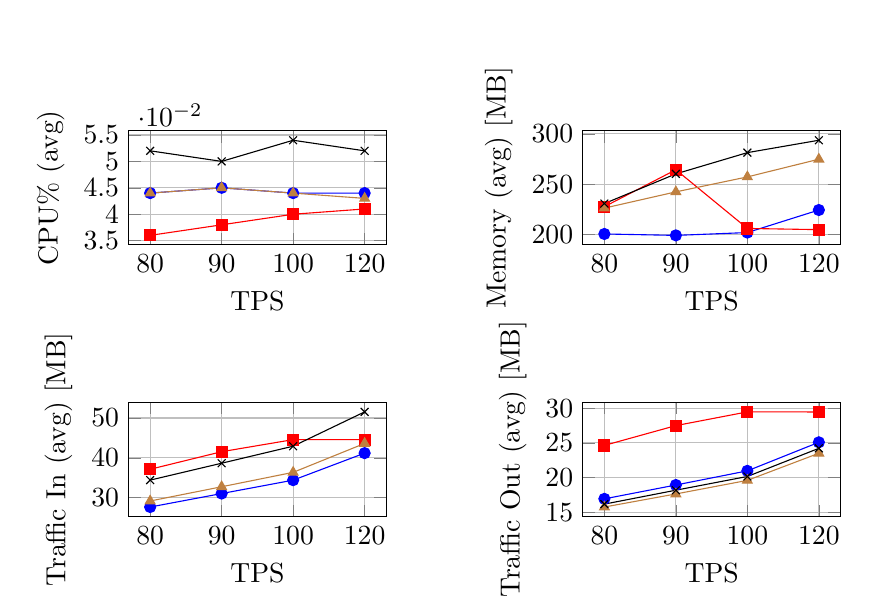
\begin{tikzpicture}
			\begin{groupplot}[
				group style={
					group name=my plots,
					group size=2 by 2,
					xlabels at=edge bottom,
					ylabels at=edge left,
					horizontal sep=2.5cm,
					vertical sep=2cm,
				},
				symbolic x coords={80, 90, 100, 120},
				xtick=data,
				width=0.4\linewidth,
				height=0.25\linewidth,
				grid=major
			]

				% CPU Usage Plot
				\nextgroupplot[legend to name=testLegend4, xlabel={TPS}, ylabel={CPU\% (avg)}]
				\addplot[blue, mark=*] coordinates {(80, 0.044) (90, 0.045) (100, 0.044) (120, 0.044)};
				\addplot[red, mark=square*] coordinates {(80, 0.036) (90, 0.038) (100, 0.040) (120, 0.041)};
				\addplot[brown, mark=triangle*] coordinates {(80, 0.044) (90, 0.045) (100, 0.044) (120, 0.043)};
				\addplot[black, mark=x] coordinates {(80, 0.052) (90, 0.050) (100, 0.054) (120, 0.052)};

				% Memory Usage Plot
				\nextgroupplot[legend to name=testLegend4, xlabel={TPS}, ylabel={Memory (avg) [MB]}]
				\addplot[blue, mark=*] coordinates {(80, 200.600) (90, 199.200) (100, 202.000) (120, 224.400)};
				\addplot[red, mark=square*] coordinates {(80, 227.700) (90, 264.400) (100, 206.100) (120, 204.900)};
				\addplot[brown, mark=triangle*] coordinates {(80, 226.286) (90, 242.429) (100, 257.286) (120, 274.857)};
				\addplot[black, mark=x] coordinates {(80, 230.800) (90, 260.300) (100, 281.400) (120, 293.700)};

				% Traffic In Plot
				\nextgroupplot[legend to name=testLegend4, xlabel={TPS}, ylabel={Traffic In (avg) [MB]}]
				\addplot[blue, mark=*] coordinates {(80, 27.660) (90, 31.040) (100, 34.400) (120, 41.180)};
				\addplot[red, mark=square*] coordinates {(80, 37.130) (90, 41.540) (100, 44.570) (120, 44.570)};
				\addplot[brown, mark=triangle*] coordinates {(80, 29.171) (90, 32.743) (100, 36.357) (120, 43.614)};
				\addplot[black, mark=x] coordinates {(80, 34.410) (90, 38.650) (100, 42.920) (120, 51.530)};

				% Traffic Out Plot
				\nextgroupplot[legend to name=testLegend4, xlabel={TPS}, ylabel={Traffic Out (avg) [MB]}]
				\addplot[blue, mark=*] coordinates {(80, 16.920) (90, 18.920) (100, 20.960) (120, 25.080)};
				\addplot[red, mark=square*] coordinates {(80, 24.630) (90, 27.490) (100, 29.470) (120, 29.460)};
				\addplot[brown, mark=triangle*] coordinates {(80, 15.743) (90, 17.629) (100, 19.586) (120, 23.500)};
				\addplot[black, mark=x] coordinates {(80, 16.160) (90, 18.170) (100, 20.150) (120, 24.210)};

				% Legend Entries
				\addlegendentry{5 Orgs 1 Peer}
				\addlegendentry{5 Orgs 2 Peers}
				\addlegendentry{7 Orgs 1 Peer}
				\addlegendentry{10 Orgs 1 Peer}
			\end{groupplot}
		\end{tikzpicture}
		\ref{testLegend4}
		\caption{Resource Usage for peers on CreateVehicle.}
		\label{fig:createvehiclepeerru}
	\end{center}
\end{figure}
Figure \ref{fig:createvehiclepeerru}
shows the peers resource utilization for CreateVehicle chaincode, CPU usage remains low and steady across all configurations,
indicating no significant strain on processing resources. Memory usage, however, shows a gradual increase with TPS, especially for
configurations with more organizations, such as 10 Orgs 1 Peer, which reaches nearly 294 MB at 120 TPS. This pattern suggests that higher
TPS rates and more complex network setups require more memory. Both inbound and outbound traffic also increase with TPS, with Traffic in and
Traffic Out showing the highest values in the 10 Orgs 1 Peer configuration, indicating a rise in data transfer requirements for larger
network setups at higher transaction rates. Overall, the results highlight that memory and network demands grow with increased TPS and
network complexity, while CPU usage remains stable.
\begin{table}[H]
	\centering
	\footnotesize
	\tiny
	\caption{Resource Usage for peers on QueryVehicle.}
	\label{tab:queryvehiclepeerru}
	\begin{tabularx}{\textwidth}
	{>{\centering\arraybackslash}X|>{\centering\arraybackslash}X|>{\centering\arraybackslash}X|>{\centering\arraybackslash}X|
			>{\centering\arraybackslash}X|>{\centering\arraybackslash}X|>{\centering\arraybackslash}X}
		\toprule
		\textbf{No. Orgs} & \textbf{No. Peers} & \textbf{TPS} & \textbf{CPU\% (avg)} & \textbf{Memory (avg) [MB]} &
		\textbf{Traffic In (avg) [MB]} & \textbf{Traffic Out (avg) [MB]} \\
		\midrule
		\multirow{4}{*}{\textbf{5}} & \multirow{2}{*}{\textbf{1}}
		& 130 & 0.057 & 205.200 & 78.320 & 43.840 \\
		\cline{3-7}
		& & 140 & 0.054 & 235.600 & 76.100 &
		42.640 \\
		\cline{2-7}
		& \multirow{2}{*}{\textbf{2}}
		& 130 & 0.053 & 273.900 & 99.620 & 62.780
		\\
		\cline{3-7}
		& & 140 & 0.052 & 281.700 & 98.680 &
		62.180 \\
		\midrule
		\multirow{2}{*}{\textbf{7}} & \multirow{2}{*}{\textbf{1}}
		& 130 & 0.071 & 242.714 & 76.271 & 36.943 \\
		\cline{3-7}
		& & 140 & 0.069 & 247.857 & 72.100 &
		35.043 \\
		\midrule
		\multirow{2}{*}{\textbf{10}} & \multirow{2}{*}{\textbf{1}}
		& 130 & 0.072 & 266.100 & 85.470 & 35.760 \\
		\cline{3-7}
		& & 140 & 0.072 & 277.200 & 84.250 &
		35.300 \\
		\bottomrule
	\end{tabularx}
\end{table}
\begin{figure}[H]
	\begin{center}
		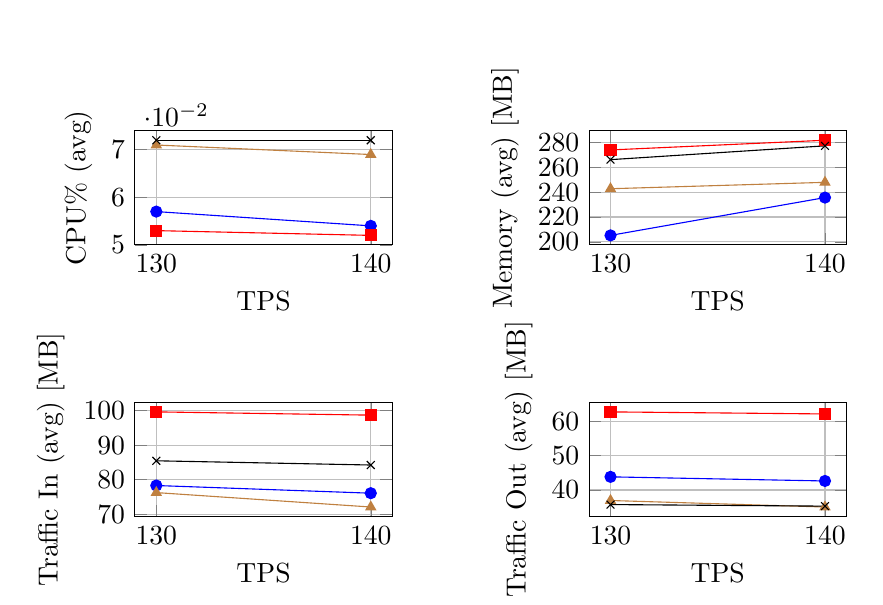
\begin{tikzpicture}
			\begin{groupplot}[
				group style={
					group name=my plots,
					group size=2 by 2,
					xlabels at=edge bottom,
					ylabels at=edge left,
					horizontal sep=2.5cm,
					vertical sep=2cm,
				},
				symbolic x coords={130, 140},
				xtick=data,
				width=0.4\linewidth,
				height=0.25\linewidth,
				grid=major
			]

				% CPU Usage Plot
				\nextgroupplot[legend to name=testLegend5, xlabel={TPS}, ylabel={CPU\% (avg)}]
				\addplot[blue, mark=*] coordinates {(130, 0.057) (140, 0.054)};
				\addplot[red, mark=square*] coordinates {(130, 0.053) (140, 0.052)};
				\addplot[brown, mark=triangle*] coordinates {(130, 0.071) (140, 0.069)};
				\addplot[black, mark=x] coordinates {(130, 0.072) (140, 0.072)};

				% Memory Usage Plot
				\nextgroupplot[legend to name=testLegend5, xlabel={TPS}, ylabel={Memory (avg) [MB]}]
				\addplot[blue, mark=*] coordinates {(130, 205.200) (140, 235.600)};
				\addplot[red, mark=square*] coordinates {(130, 273.900) (140, 281.700)};
				\addplot[brown, mark=triangle*] coordinates {(130, 242.714) (140, 247.857)};
				\addplot[black, mark=x] coordinates {(130, 266.100) (140, 277.200)};

				% Traffic In Plot
				\nextgroupplot[legend to name=testLegend5, xlabel={TPS}, ylabel={Traffic In (avg) [MB]}]
				\addplot[blue, mark=*] coordinates {(130, 78.320) (140, 76.100)};
				\addplot[red, mark=square*] coordinates {(130, 99.620) (140, 98.680)};
				\addplot[brown, mark=triangle*] coordinates {(130, 76.271) (140, 72.100)};
				\addplot[black, mark=x] coordinates {(130, 85.470) (140, 84.250)};

				% Traffic Out Plot
				\nextgroupplot[legend to name=testLegend5, xlabel={TPS}, ylabel={Traffic Out (avg) [MB]}]
				\addplot[blue, mark=*] coordinates {(130, 43.840) (140, 42.640)};
				\addplot[red, mark=square*] coordinates {(130, 62.780) (140, 62.180)};
				\addplot[brown, mark=triangle*] coordinates {(130, 36.943) (140, 35.043)};
				\addplot[black, mark=x] coordinates {(130, 35.760) (140, 35.300)};

				% Legend Entries
				\addlegendentry{5 Orgs 1 Peer}
				\addlegendentry{5 Orgs 2 Peers}
				\addlegendentry{7 Orgs 1 Peer}
				\addlegendentry{10 Orgs 1 Peer}
			\end{groupplot}
		\end{tikzpicture}
		\ref{testLegend5}
		\caption{Resource Usage for peers on QueryVehicle.}
		\label{fig:queryvehiclepeerru}
	\end{center}
\end{figure}
Figure \ref{fig:queryvehiclepeerru}
shows the results for peers resource utilization on the QueryVehicle chaincode which show that CPU usage remains steady and low
across configurations, indicating that CPU resources are not a primary limiting factor. However, memory usage varies more significantly with
the configuration, with 5 Orgs 2 Peers and 10 Orgs 1 Peer reaching the highest values, suggesting increased memory demands for more complex
setups. Network traffic shows a slight decrease in Traffic in and Traffic Out as TPS increases, due to the increase in the number of
organizations and the impact it has on the throughput. Overall, the findings highlight that while memory usage scales with configuration
complexity, CPU and network demands remain more stable, allowing for more predictable performance at these higher transaction rates.

\subsubsection{Orderer Evaluation}
\begin{table}[H]
	\centering
	\footnotesize
	\tiny
	\caption{Resource Usage for orederers on CreateVehicle chaincode.}
	\label{tab:createvehicleordererru}
	\begin{tabularx}{\textwidth}
	{>{\centering\arraybackslash}X|>{\centering\arraybackslash}X|>{\centering\arraybackslash}X|>{\centering\arraybackslash}X|
			>{\centering\arraybackslash}X|>{\centering\arraybackslash}X|>{\centering\arraybackslash}X}
		\toprule
		\textbf{No. Orgs} & \textbf{No. Peers} & \textbf{TPS} & \textbf{CPU\% (avg)} & \textbf{Memory (avg) [MB]} &
		\textbf{Traffic In (avg) [MB]} & \textbf{Traffic Out (avg) [MB]} \\
		\midrule
		\multirow{8}{*}{\textbf{5}} & \multirow{4}{*}{\textbf{1}}
		& 80 & 0.007 & 72.700 & 19.300 & 39.433 \\
		\cline{3-7}
		& & 90 & 0.006 & 72.567 & 21.667 &
		44.367 \\
		\cline{3-7}
		& & 100 & 0.006 & 73.700 & 24.267 &
		49.433 \\
		\cline{3-7}
		& & 120 & 0.006 & 76.933 & 28.867 &
		59.100 \\
		\cline{2-7}
		& \multirow{4}{*}{\textbf{2}}
		& 80 & 0.009 & 80.567 & 19.267 & 64.733
		\\
		\cline{3-7}
		& & 90 & 0.009 & 91.867 & 21.667 &
		72.833 \\
		\cline{3-7}
		& & 100 & 0.010 & 76.733 & 23.300 &
		78.133 \\
		\cline{3-7}
		& & 120 & 0.010 & 81.933 & 23.333 &
		78.133 \\
		\midrule
		\multirow{4}{*}{\textbf{7}} & \multirow{4}{*}{\textbf{1}}
		& 80 & 0.007 & 82.700 & 22.433 & 57.600 \\
		\cline{3-7}
		& & 90 & 0.008 & 79.767 & 25.167 &
		64.733 \\
		\cline{3-7}
		& & 100 & 0.008 & 95.333 & 27.933 &
		71.933 \\
		\cline{3-7}
		& & 120 & 0.008 & 96.400 & 33.467 &
		86.167 \\
		\midrule
		\multirow{4}{*}{\textbf{10}} & \multirow{4}{*}{\textbf{1}}
		& 80 & 0.006 & 81.467 & 28.467 & 96.067 \\
		\cline{3-7}
		& & 90 & 0.006 & 94.300 & 31.933 &
		108.033 \\
		\cline{3-7}
		& & 100 & 0.006 & 101.467 & 35.700 &
		119.967 \\
		\cline{3-7}
		& & 120 & 0.005 & 208.667 & 42.667 &
		143.900 \\
		\bottomrule
	\end{tabularx}
\end{table}
\begin{figure}[H]
	\begin{center}
		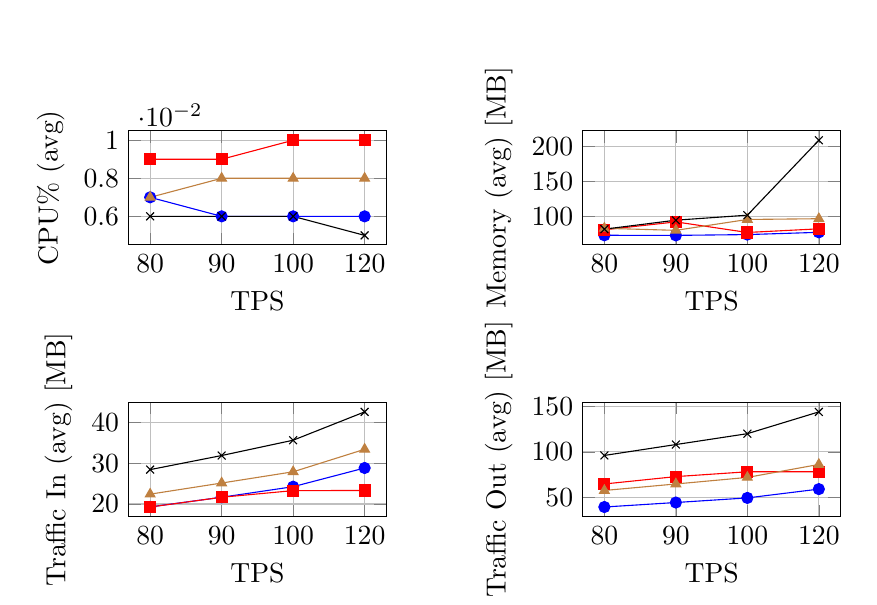
\begin{tikzpicture}
			\begin{groupplot}[
				group style={
					group name=my plots,
					group size=2 by 2,
					xlabels at=edge bottom,
					ylabels at=edge left,
					horizontal sep=2.5cm,
					vertical sep=2cm,
				},
				symbolic x coords={80, 90, 100, 120},
				xtick=data,
				width=0.4\linewidth,
				height=0.25\linewidth,
				grid=major
			]

				% CPU Usage Plot
				\nextgroupplot[legend to name=testLegend6, xlabel={TPS}, ylabel={CPU\% (avg)}]
				\addplot[blue, mark=*] coordinates {(80, 0.007) (90, 0.006) (100, 0.006) (120, 0.006)};
				\addplot[red, mark=square*] coordinates {(80, 0.009) (90, 0.009) (100, 0.010) (120, 0.010)};
				\addplot[brown, mark=triangle*] coordinates {(80, 0.007) (90, 0.008) (100, 0.008) (120, 0.008)};
				\addplot[black, mark=x] coordinates {(80, 0.006) (90, 0.006) (100, 0.006) (120, 0.005)};

				% Memory Usage Plot
				\nextgroupplot[legend to name=testLegend6, xlabel={TPS}, ylabel={Memory (avg) [MB]}]
				\addplot[blue, mark=*] coordinates {(80, 72.700) (90, 72.567) (100, 73.700) (120, 76.933)};
				\addplot[red, mark=square*] coordinates {(80, 80.567) (90, 91.867) (100, 76.733) (120, 81.933)};
				\addplot[brown, mark=triangle*] coordinates {(80, 82.700) (90, 79.767) (100, 95.333) (120, 96.400)};
				\addplot[black, mark=x] coordinates {(80, 81.467) (90, 94.300) (100, 101.467) (120, 208.667)};

				% Traffic In Plot
				\nextgroupplot[legend to name=testLegend6, xlabel={TPS}, ylabel={Traffic In (avg) [MB]}]
				\addplot[blue, mark=*] coordinates {(80, 19.300) (90, 21.667) (100, 24.267) (120, 28.867)};
				\addplot[red, mark=square*] coordinates {(80, 19.267) (90, 21.667) (100, 23.300) (120, 23.333)};
				\addplot[brown, mark=triangle*] coordinates {(80, 22.433) (90, 25.167) (100, 27.933) (120, 33.467)};
				\addplot[black, mark=x] coordinates {(80, 28.467) (90, 31.933) (100, 35.700) (120, 42.667)};

				% Traffic Out Plot
				\nextgroupplot[legend to name=testLegend6, xlabel={TPS}, ylabel={Traffic Out (avg) [MB]}]
				\addplot[blue, mark=*] coordinates {(80, 39.433) (90, 44.367) (100, 49.433) (120, 59.100)};
				\addplot[red, mark=square*] coordinates {(80, 64.733) (90, 72.833) (100, 78.133) (120, 78.133)};
				\addplot[brown, mark=triangle*] coordinates {(80, 57.600) (90, 64.733) (100, 71.933) (120, 86.167)};
				\addplot[black, mark=x] coordinates {(80, 96.067) (90, 108.033) (100, 119.967) (120, 143.900)};

				% Legend Entries
				\addlegendentry{5 Orgs 1 Peer}
				\addlegendentry{5 Orgs 2 Peers}
				\addlegendentry{7 Orgs 1 Peer}
				\addlegendentry{10 Orgs 1 Peer}
			\end{groupplot}
		\end{tikzpicture}
		\ref{testLegend6}
		\caption{Resource Usage for orderers on CreateVehicle chaincode.}
		\label{fig:createvehicleordererru}
	\end{center}
\end{figure}
Figure \ref{fig:createvehicleordererru}
shows resource utilization for the orderer nodes for the CreateVehicle chaincode scale with both TPS and the number of
organizations, particularly in terms of memory usage and network traffic. CPU usage remains low across all configurations, suggesting it is
not a primary bottleneck. However, as TPS increases, configurations with more organizations, especially 10 Orgs 1 Peer, experience
significant spikes in memory usage and both inbound and outbound network traffic, generally, traffic increase with the number of
organizations as orederers communication cost will increase to communicate with all of them. These findings highlight that while CPU
resources are sufficient, memory and network capacity may become constraints in larger, high-throughput setups, suggesting a need for
optimizations to support scalability.

As mentioned above, Caliper is intended to be used on real enterprise projects and for development cases, it
was used for our framework to provide us with an insight of the framework performance and challenges that might occur
, however, after tracing and debugging the high latency cause. We discovered that it was due to the high
number of containers in the network, which leads the network bandwidth to be a bottleneck as most of the
latency time is on google Remote Procedure Calls (gRPC) calls between nodes while CPU usage highest value was 70%. 

\subsection{Performance Evaluation Using HL Tape}
HL Tape is lightweight benchmarking tool developed by HL foundation for HL fabric to measure performance. Unlike Caliper, tape is designed
to be used as a stress testing tool, which measure who the network handles high volume of transactions. It is mainly focused on throughput
and suitable for development purposes when quick feedback is required, also it is better suited than caliper for limited resources and
single machine deployments. As stated above, tape is lightweight and requires a simple configuration. For our evaluation, the number of
transactions will be 10000 and commitOnly mode will be used. As mentioned in 4.3.1 Caliper is not suitable for single machine deployments
and due to the bottleneck caused by the network bandwidth, commitOnly is used to measure the throughput using the committing phase by
isolating this phase from the delays produced by the network congestion. These results would provide a valuable insight into the framework
performance under the load when deployed on a real network and measure the throughput with an accuracy higher than caliper.
\begin{table}[H]
	\centering
	\footnotesize
	\tiny
	\caption{Performance Metrics for Tape on CreateVehicle chaincode}
	\label{tab:tapecreatevehiclepm}
	\begin{tabularx}{\textwidth}
	{>{\centering\arraybackslash}X|>{\centering\arraybackslash}X|>{\centering\arraybackslash}X|>{\centering\arraybackslash}X|
			>{\centering\arraybackslash}X}
		\toprule
		\textbf{Batch Timeout (S)} & \textbf{Max Message Count} & \textbf{No. of Transactions} & \textbf{Duration (S)} & \textbf{TPS} \\
		\midrule
		\multirow{5}{*}{1}           & 100                        & 10000                        & 9.67                  & 1033.90      \\
		\cline{2-5}
		& 250                        & 10000                        & 8.27                  & 1208.91      \\
		\cline{2-5}
		& 500                        & 10000                        & 6.81                  & 1467.81      \\
		\cline{2-5}
		& 750                        & 10000                        & 8.74                  & 1144.03      \\
		\cline{2-5}
		& 1000                       & 10000                        & 6.82                  & 1466.65      \\
		\midrule
		\multirow{5}{*}{2}           & 100                        & 10000                        & 7.20                  & 1388.70      \\
		\cline{2-5}
		& 250                        & 10000                        & 4.51                  & 2216.90      \\
		\cline{2-5}
		& 500                        & 10000                        & 4.77                  & 2096.21      \\
		\cline{2-5}
		& 750                        & 10000                        & 7.57                  & 1321.79      \\
		\cline{2-5}
		& 1000                       & 10000                        & 6.94                  & 1441.20      \\
		\midrule
		\multirow{5}{*}{5}           & 100                        & 10000                        & 6.03                  & 1658.33      \\
		\cline{2-5}
		& 250                        & 10000                        & 5.10                  & 1962.48      \\
		\cline{2-5}
		& 500                        & 10000                        & 8.14                  & 1227.90      \\
		\cline{2-5}
		& 750                        & 10000                        & 8.02                  & 1247.21      \\
		\cline{2-5}
		& 1000                       & 10000                        & 7.12                  & 1404.73      \\
		\midrule
		\multirow{5}{*}{10}          & 100                        & 10000                        & 8.33                  & 1199.87      \\
		\cline{2-5}
		& 250                        & 10000                        & 7.97                  & 1254.56      \\
		\cline{2-5}
		& 500                        & 10000                        & 7.99                  & 1251.22      \\
		\cline{2-5}
		& 750                        & 10000                        & 12.84                 & 778.69       \\
		\cline{2-5}
		& 1000                       & 10000                        & 4.99                  & 2004.87      \\
		\bottomrule
	\end{tabularx}
\end{table}


\begin{figure}[H]
	\centering
	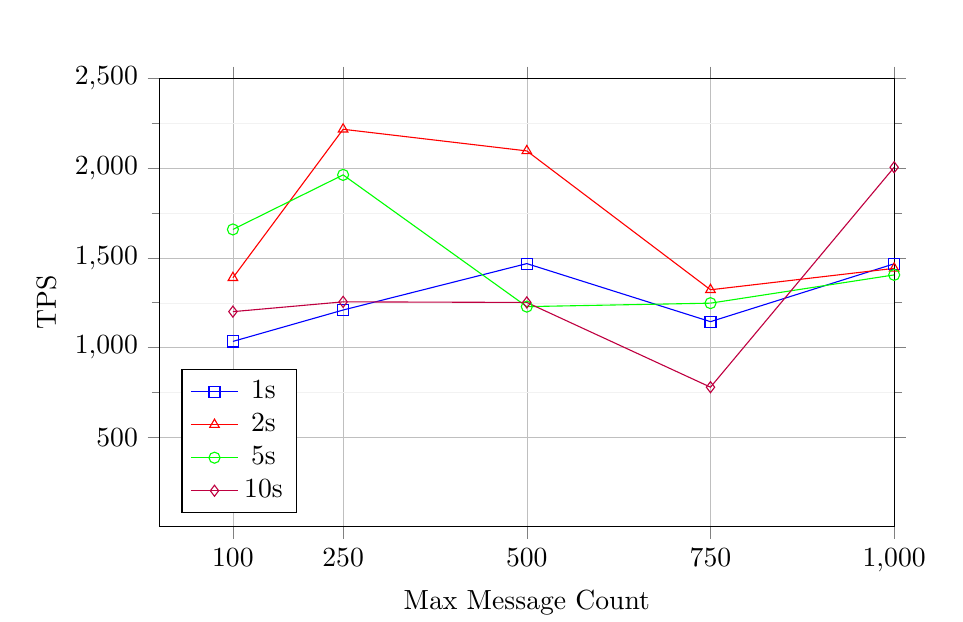
\begin{tikzpicture}
		\begin{axis}[
			width=0.9\textwidth,
			height=0.6\textwidth,
			xlabel={Max Message Count},
			ylabel={TPS},
			xmin=0, xmax=1000,
			ymin=0, ymax=2500,
			xtick={100, 250, 500, 750, 1000},
			ytick={500, 1000, 1500, 2000, 2500},
			legend pos=south west,
			legend style={anchor=south west, cells={align=left}},
			grid=both,
			grid style={line width=.1pt, draw=gray!10},
			major grid style={line width=.2pt,draw=gray!50},
			minor tick num=1,
			tick align=outside
		]

			% Plot data for each Batch Timeout value
			\addplot[
				color=blue, mark=square
			]
			coordinates {
				(100, 1033.90) (250, 1208.91) (500, 1467.81) (750, 1144.03) (1000, 1466.65)
			};
			\addlegendentry{1s}

			\addplot[
				color=red, mark=triangle
			]
			coordinates {
				(100, 1388.70) (250, 2216.90) (500, 2096.21) (750, 1321.79) (1000, 1441.20)
			};
			\addlegendentry{2s}

			\addplot[
				color=green, mark=o
			]
			coordinates {
				(100, 1658.33) (250, 1962.48) (500, 1227.90) (750, 1247.21) (1000, 1404.73)
			};
			\addlegendentry{5s}

			\addplot[
				color=purple, mark=diamond
			]
			coordinates {
				(100, 1199.87) (250, 1254.56) (500, 1251.22) (750, 778.69) (1000, 2004.87)
			};
			\addlegendentry{10s}

		\end{axis}
	\end{tikzpicture}
	\caption{Performance Metrics for Tape on CreateVehicle chaincode}
	\label{fig:tapecreatevehiclepm}
\end{figure}
As figure \ref{fig:tapecreatevehiclepm} shows, the framework is capable of achieving around 2200 TPS which would yield an efficient performance. The fabric
configurations for channel such as block time, message count, and max size can be updated on an existing channel and does not require a new
one, framework should be monitored consistently, and configurations should be updated accordingly to maintain most efficient performance and
resource utilization.

\section{Conclusion}
The automotive industry is one of the biggest in the world, which increases the importance of ensuring integrity and trust in the vehicle
market. In this research, we presented a new framework based on HL fabric BC to record and secure all events in the vehicle lifecycle to
ensure trust between sellers and buyers in the market. Based on the evaluation results, our framework could provide significant value to the
market.

The framework functionality was assessed using manual testing and HL Explorer. Results showed that all test scenarios were successfully
executed with the framework operating without any critical issues. This demonstrates that the integration between framework parts is
reliable. Additionally, scalability was tested using HL caliper with a variation of organizations. Results show a potential for scaling by
either adding a new server for each organization or adding new peers to an organization. However, the framework gained a significant spike
when additional peers were added. Furthermore, latency was measured using HL caliper, although it should be noted that it was not intended
for single-machine benchmarking. Despite that, the results provided valuable insight. Latency was relatively high, which is explained by the
deployment on a single machine, also, network bandwidth was a limitation that caused the high latency and affected the overall performance,
nevertheless, network bandwidth should be taken into consideration when deploying to a real network. Finally, several security measures were
implemented, including TLS encryption, rate controller, and the use of spring security and JWT to handle authorization and authentication.
Despite these measures providing adequate protection, continuous improvements are essential to maintaining network integrity.

In future research, we would use security keys such as yubikey to store user certificates and explore the impact of using other languages
such as Go language and Node JS and databases such as level DB. OpenSearch can also be used to store and query images, it has the ability to
handle tremendous amounts of data and perform complex queries which can enhance image retrieval. Furthermore, Machine Learning (ML) and
Artificial Intelligence (AI) could be implemented to fairly estimate vehicle prices based on information retrieved from the framework.

\printbibliography[heading=bibintoc]

\end{document}

%%
%% End of file `iaesarticle.tex'. 